\newpage

\section{Connections To Variational EM}

\label{app:connections}

In this Appendix, we derive $J_{\pi-\text{Distill}}$ using a variational perspective. Specifically, we show how $J_{\pi-\text{Distill}}$ can be seen as a joint EM algorithm where E and M are done simultaneously.  

Traditional variational-EM aims to fit a parameterized distribution $\piS$ onto a target posterior $\pi^*$. An assumption this framework makes is that using $\piS$ to approximate  $\pi^*$ may be suboptimal, rather, leveraging an approximate posterior $\piTthetafull$ conditioned on additional information can make the approximation easier. This is true when $\piT$ can sample from high-reward modes that $\piS$ cannot, therefore making optimization via RL impossible for $\piS$. We visualize the procedure in \Cref{fig:variational-em-figure}
\subsection{Variational EM}

\begin{figure}[h]
    \centering
    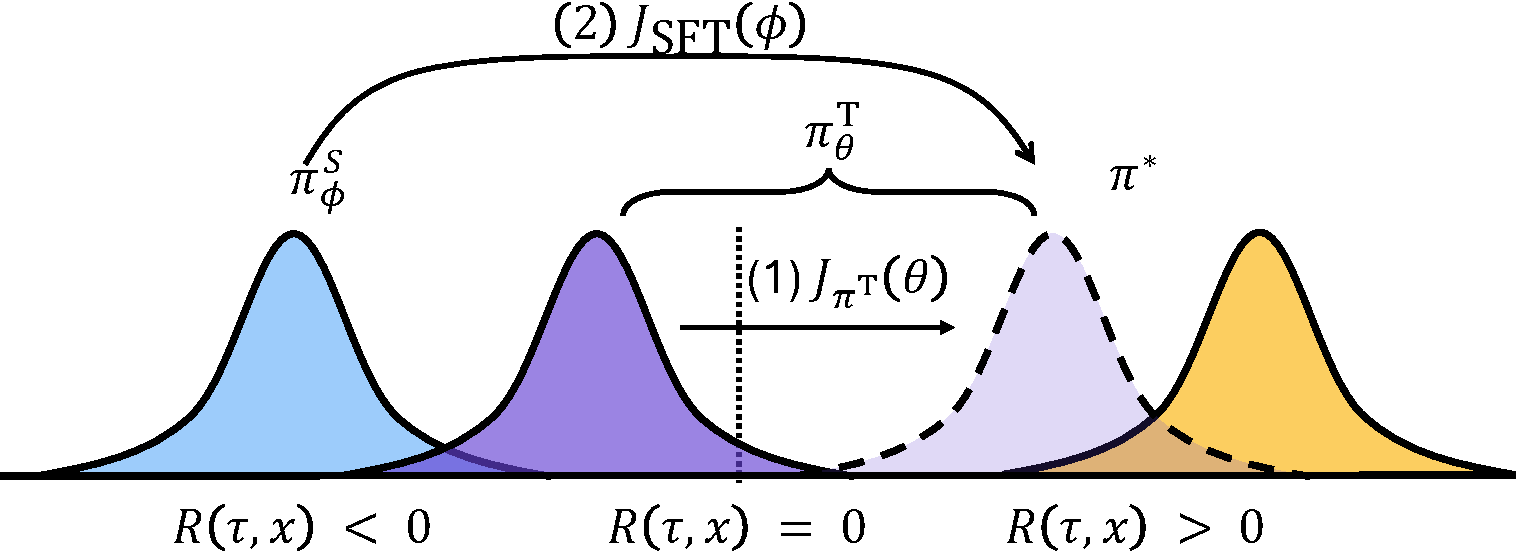
\includegraphics[width=1\linewidth]{figures/CURVESpdf-pages.pdf}
    \caption{\textbf{Illustration of the Variational EM procedure for policy optimization}. The initial student policy, $\pi_{\theta}^{S}$, lacks support over trajectories with positive rewards ($R(\mathbf{o}, \mathbf{s}) > 0$), preventing direct improvement. To address this: (1) the teacher policy $\pi_{\theta}^{T}$ is optimized via $J_{\text{Teacher}}(\theta)$ to sample successful traces and approximate the optimal policy $\pi^*$; (2) the student policy is then updated via $J_{\text{SFT}}(\theta)$ to distill the knowledge from the teacher. While this two-step procedure is principled, it is computationally inefficient due to the requirement of maintaining dual parameter sets and distinct training phases. In contrast, $\pi$-Distill simplifies this pipeline into a single-phase process, providing superior performance with reduced complexity.} 
    \label{fig:variational-em-figure}
\end{figure}
\label{app:derivation-j-pi-h}

\paragraph{E-step $J_{\text{Teacher}}$.}

We first define the target posterior we want to fit, $\pi^*$, as a reward-tilted posterior relative to the reference policy $\pi_{\text{ref}}$. For a given state $\mathbf{s}$, we define:
\begin{equation}
    \pi^*(\mathbf{o} \mid \mathbf{s}) = \frac{\pi_{\text{ref}}(\mathbf{o} \mid \mathbf{s}) \exp(R(\mathbf{o}, \mathbf{s}))}{Z}
\end{equation}
where $Z = \sum_{\mathbf{o'}} \pi_{\text{ref}}(\mathbf{o'} \mid \mathbf{s}_0) \exp(R(\mathbf{o'}, \mathbf{s}))$ is the partition function and $\mathbf{o}=(\mathbf{z},\mathbf{a})$ consists of internal reasoning tokens $\mathbf{z}$ and action tokens $\mathbf{a}$.

The partition function makes this distribution intractable, but it can be approximated using a variational posterior $\piTthetafull$ conditioned on privileged information $\mathbf{I}$. We optimize parameters $\theta$ by minimizing the reverse KL between the variational distribution and the target policy:

\begin{align}
\label{eq:j_teacher}
J_{\text{Teacher}}(\theta) 
&= - D_{\text{KL}}\!\left(\piTthetafull \parallel \pi^*(\cdot \mid \mathbf{s}) \right) \nonumber \\
&= - \mathbb{E}_{\substack{\mathbf{o} \sim \piTthetafull \\ \mathbf{s} \sim P}} \left[ \log \frac{\piTthetafull}{\pi^*(\mathbf{o} \mid \mathbf{s})} \right] \nonumber \\
&= \mathbb{E}_{\substack{\mathbf{o} \sim \piTthetafull \\ \mathbf{s} \sim P}} \left[ \log \pi^*(\mathbf{o} \mid \mathbf{s}) - \log \piTthetafull \right]
\end{align}

Substituting the definition of $\pi^*$ into the equation:
\begin{align}
\label{eq:teacher_derivation}
J_{\text{Teacher}}(\theta) 
&= \mathbb{E}_{\substack{\mathbf{o} \sim \piTthetafull \\ \mathbf{s} \sim P}} \left[ \log \left( \frac{\pi_{\text{ref}}(\mathbf{o} \mid \mathbf{s}) \exp(R(\mathbf{o}, \mathbf{s}))}{Z} \right) - \log \piTthetafull \right] \nonumber \\
&= \mathbb{E}_{\substack{\mathbf{o} \sim \piTthetafull \\ \mathbf{s} \sim P}} \left[ R(\mathbf{o}, \mathbf{s}) + \log \pi_{\text{ref}}(\mathbf{o} \mid \mathbf{s}) - \log \piTthetafull - \log Z \right] \nonumber \\
&= \mathbb{E}_{\substack{\mathbf{o} \sim \piTthetafull \\ \mathbf{s} \sim P}} \left[ R(\mathbf{o}, \mathbf{s}) - \left( \log \piTthetafull - \log \pi_{\text{ref}}(\mathbf{o} \mid \mathbf{s}) \right) \right] - \log Z \nonumber \\
&\propto \mathbb{E}_{\substack{\mathbf{o} \sim \piTthetafull \\ \mathbf{s} \sim P}} [ R(\mathbf{o}, \mathbf{s}) ] - D_{\text{KL}}\!\left( \piTthetafull \parallel \pi_{\text{ref}}(\cdot \mid \mathbf{s}) \right)
\end{align}

Since $\log Z$ depends only on the context $\mathbf{s}$, it is constant with respect to $\theta$ and can be omitted.

\paragraph{M-step $J_{\text{SFT}}$.}
If $\pi^*$ were a tractable distribution, we could directly fit the target policy by minimizing the forward KL divergence, $D_{\text{KL}}(\pi^* \parallel \piStheta)$, corresponding to standard SFT. Since $\pi^*$ is intractable, we instead substitute it with our learned approximation $\piTtheta$, yielding the following objective:
\begin{align}
\label{eq:sft}
    J_{\text{SFT}}(\theta) = \mathbb{E}_{\substack{\mathbf{o} \sim \piTthetafull \\ \mathbf{s} \sim P}} \left[ \log \piSthetafull \right].
\end{align}

Traditionally, one would either first fit $\piTtheta$ to convergence and use it to fit $\piStheta$, or alternate between training the teacher and student. Regardless, this process requires two separate models and can be difficult to optimize. Our implementation is a modified version of \citet{zhou2025variationalreasoninglanguagemodels}, where the modifications are specific to our multi-turn setting, where no ground truth is provided. 

% \paragraph{Variational EM viewpoint.}
% If $\pi^h_\theta$ were a good approximation of $\pi^*$, we could then fit an unconditioned (deployment-time) policy $\pi_\phi(\mathbf{o}\mid s)$ by minimizing the forward KL
% $D_{\mathrm{KL}}(\pi^*\|\pi_\phi)$.
% Since $\pi^*$ is intractable, a standard approximation is to replace it with samples from the learned guide and perform maximum-likelihood training:
% \begin{align}
% \label{eq:j_sft}
% J_{\mathrm{SFT}}(\phi)
% = \mathbb{E}_{\mathbf{o}\sim \pi^{h*}_\theta(\cdot\mid s,h)}
% \big[\log \pi_\phi(\mathbf{o}\mid s)\big],
% \end{align}
% where $\pi^{h*}_\theta$ denotes the (approximately) optimized guide. This yields a two-step procedure reminiscent of variational EM: (E-step) optimize the guide via \Cref{eq:j_pih}, then (M-step) distill into $\pi_\phi$ via \Cref{eq:j_sft}. \Cref{fig:curves-moving} illustrates this workflow. \EP{We should mention (perhaps as a footnote) that we also tried iterative EM-style alternation and found it ineffective in these agentic tasks.}

\subsection{Failures of Variational EM.} 
\label{app:em-failure}
\begin{figure}[ht]
    \centering
    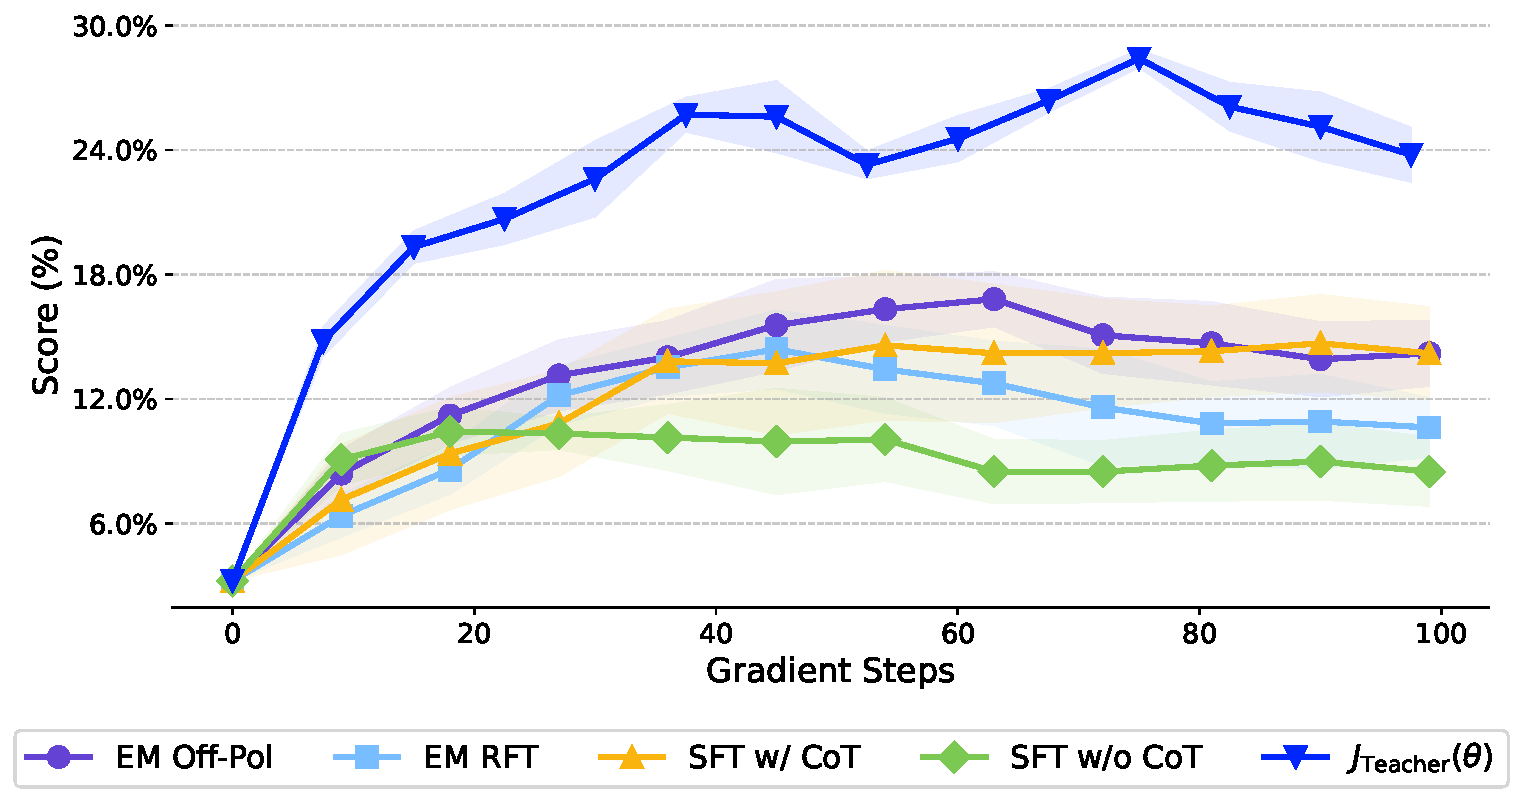
\includegraphics[width=0.95\linewidth]{figures/sft_plot.pdf}
    \caption{\textbf{Performance of Sequential EM variants on $\tau$-Bench Retail (\texttt{Qwen3-8B})}. We compare these methods against SFT baselines. While standard EM RFT (light blue) fails to match SFT w/ CoT (yellow), replacing RFT with off-policy RL (EM Off-Pol, purple) successfully allows for EM to outperform SFT w CoT. The strongest performance comes from $J_{\text{Teacher}}(\theta)$ (dark blue), demonstrating that parameter sharing between the teacher and student yields the most effective transfer. Shaded regions indicate standard error across 3 seeds.}
    \label{fig:em-plots}
\end{figure}
\newpage
\label{app:em-failure}
Our initial efforts focused on making variational EM work, similar in spirit to \cite{zhou2025variationalreasoninglanguagemodels}. We first document initial ideas that were unsuccessful, then we discuss the best version of EM we could find, being a sequential implementation. Finally, we discuss how these experiments ultimately motivated the design decisions for $\pi$-Distill.

\paragraph{Initial Experiments}
First, we find that setting the reference policy $\pi_{\text{ref}}$ as a copy of the current student $\piStheta$ is crucial for learning. In contrast, using the fixed base model $\pi_{\text{base}}$ as a prior significantly hinders performance (see App.~\ref{app:ref-model-ablation}).

Building on this insight, we initially explored an offline variational EM method similar to \citet{zhou2025variationalreasoninglanguagemodels}. Here, the goal is learning a CoT sampler as the variational posterior conditioned on expert traces. We do this with the following objective:
\begin{align}
J_{\text{Offline-EM}}(\theta) &= \mathbb{E}_{\mathbf{s} \sim \mathcal{D}} \left[ \log \sum_{\mathbf{z}} \piStheta(\mathbf{a}, \mathbf{z} \mid \mathbf{s}) \exp(R(\mathbf{o}, \mathbf{s})) \right] \nonumber \\
 &\propto \mathbb{E}_{\substack{\mathbf{a,s} \sim \mathcal{D}, \mathbf{z} \sim \piTtheta }} \left[ R(\mathbf{o}, \mathbf{s}) + \log \piStheta(\mathbf{a} \mid \mathbf{z}, \mathbf{s}) \right] - D_{\text{KL}}\!\left( \piTtheta(\mathbf{z} \mid \mathbf{s}) \parallel\piStheta(\mathbf{z} \mid \mathbf{s}) \right)
\end{align}

Notice here how the states are fixed and given in the offline dataset $\mathcal{D}$. Furthermore, this setup necessitates substantial hyperparameter tuning. Beyond the standard penalty $\beta$, the algorithm requires balancing the ratio of teacher-to-student updates, managing separate optimizer states, and calibrating the dataset size sampled from the teacher. Ultimately, we find this approach hard to implement and fails in our multi-turn setting. We attribute the success of \citet{zhou2025variationalreasoninglanguagemodels} to their access to oracle answers; in our context, we find that fitting a variational posterior to suboptimal frontier model trajectories can even degrade performance. 

Our following efforts focused on training the teacher online using \Cref{eq:j_teacher}.  We try this with alternating loops between student and teacher training, but find this to be ineffective.  As we found it hard to avoid the student and teacher collapsing onto each other using this setup. Ultimately, we found a sequential version of EM worked best, though it still requires specific adjustments to achieve optimal performance.


\paragraph{Sequential EM.}
We turn to Sequential EM after ruling out offline and alternating approaches. However, we find standard implementations remain unreliable for complex agentic tasks. Here, we analyze the limitations of standard EM and how they ultimately motivated $\pi$-Distill.

For this analysis, we use $\tau$-Bench Retail with \texttt{Qwen3-8B} using self-generated hints to train the teacher as this configuration performs best (see \S~\ref{sec:hint-ablations}). We compare sequential EM, where we first train the teacher and then perform SFT on successful trajectories (Rejection Fine-tuning or RFT), against SFT with and without CoT. We note that here it would be sufficient to outperform SFT without CoT as we assume no access to the internal CoT of the frontier model, thus in practice, sequential EM could replace the traditional SFT phase before RL.

We report results in \Cref{fig:em-plots}. First, we observe that standard Sequential EM outperforms naive SFT but lags behind training with CoT. We attribute the performance gap to the lack of negative feedback on failed trajectories. It only mimics the teacher. To address this, we replaced the RFT step with clipped off-policy RL. We find that this change enables sequential EM to outperform SFT with CoT.


Most surprisingly, in these experiments, we find that simply optimizing $J_{\text{Teacher}}(\theta)$ substantially improves the student $\piStheta$ when both teacher and student share parameters. This drastically outperforms all other baselines.

To summarize, our two main findings are that parameter sharing enables substantial transfer from teacher to student and the importance of leveraging negative traces via off-policy RL when training the student. We use these two findings to instantiate $\pi$-Distill while also simplifying the process from two training steps to a single one. 




% These empirical insights directly inform the design of $\pi$-Distill:
% \begin{finding}{Design Principles: $\pi$-Distill}
% \begin{itemize}
% \item Objective: Replacing the M-step SFT with clipped off-policy RL improves transfer by utilizing negative feedback.
% \item Architecture: Parameter sharing ($\pi^h \equiv \pi$) outperforms separate models; learning with hints directly updates the weights used for unconditioned evaluation.
% \end{itemize}
% \end{finding}



\section{On-Policy Self-Distillation $J_{\text{OPSD}}$}
\label{app:self-distill-obj}
Contrary to the prior objectives, OPSD, rather, than trying to approximate $\pi^*$ can be framed as the reverse-Kl between $\pi$ and the target conditioned policy $\pi^{T*}$, being defined as:


\begin{equation}
     \pi^*(\mathbf{o} \mid  \mathbf{s},\mathbf{I}) = \frac{\pi_{\text{ref}}(\mathbf{o} \mid \mathbf{s},\mathbf{I}) \exp(\frac{R(\mathbf{o}, \mathbf{s}))}{\beta}}{Z^h}
\end{equation}

where $Z^h = \sum_{\mathbf{o'}} \pi_{\text{ref}}^T(\mathbf{o}' \mid  \mathbf{s},\mathbf{I}) \exp(R(\mathbf{o}', \mathbf{s}))$ is the partition function.

One can then approximate this distribution directly via reverse KL, giving the following objective: 

To do this, we minimize the reverse KL between the student policy $\piStheta$ and the optimal privileged target distribution $\pi^*$:


\begin{align}
    D_{\text{KL}}(\piStheta \parallel \pi^*) &= \mathbb{E}_{\substack{\mathbf{o} \sim \piSthetafull \\ \mathbf{s} \sim P}} \left[ \log \frac{\piStheta(\mathbf{o} \mid \mathbf{s})}{\pi^*(\mathbf{o} \mid \mathbf{s}, \mathbf{I})} \right] \nonumber \\
    &= \mathbb{E}_{\substack{\mathbf{o} \sim \piSthetafull \\ \mathbf{s} \sim P}} \left[ \log \piStheta(\mathbf{o} \mid \mathbf{s}) - \log \left( \frac{\pi_{\text{ref}}(\mathbf{o} \mid\mathbf{s}, \mathbf{I}) \exp(R(\mathbf{o}, \mathbf{s})/\beta)}{Z^h} \right) \right] \nonumber \\
    &= \mathbb{E}_{\substack{\mathbf{o} \sim \piSthetafull \\ \mathbf{s} \sim P}} \left[ \log \piStheta(\mathbf{o} \mid \mathbf{s}) - \log \pi_{\text{ref}}(\mathbf{o} \mid \mathbf{s}, \mathbf{I}) - \frac{R(\mathbf{o}, \mathbf{s})}{\beta} + \log Z^h \right] \nonumber \\
    &= \mathbb{E}_{\substack{\mathbf{o} \sim \piSthetafull \\ \mathbf{s} \sim P}} \left[ - \frac{R(\mathbf{o}, \mathbf{s})}{\beta} + \log \frac{\piStheta(\mathbf{o} \mid \mathbf{s})}{\pi_{\text{ref}}(\mathbf{o} \mid  \mathbf{s}, \mathbf{I})} \right] + \log Z^h\\
    &= -\frac{1}{\beta}\mathbb{E}_{\substack{\mathbf{o} \sim \piSthetafull \\ \mathbf{s} \sim P}}
   \left[
     R(\mathbf{o},\mathbf{s})
   \right]
   + D_{\text{KL}}\!\left(
       \piStheta(\cdot \mid \mathbf{s})
       \parallel
       \pi_{\text{ref}}(\cdot \mid \mathbf{s}, \mathbf{I})
     \right)
   + \log Z^h.\\
   &\propto      -\mathbb{E}_{\substack{\mathbf{o} \sim \piSthetafull \\ \mathbf{s} \sim P}}
   \left[
     R(\mathbf{o},\mathbf{s})
   \right]
   + \beta D_{\text{KL}}\!\left(
       \piStheta(\cdot \mid \mathbf{s})
       \parallel
       \pi_{\text{ref}}(\cdot \mid \mathbf{s}, \mathbf{I})
     \right)
\end{align}

To align with $\pi$-Distill and the according to the results in App.~\ref{app:ref-model-ablation}, we set $\pi_{\text{ref}} = \piTthetafull$


% \paragraph{Failure of $J_{\text{OPSD}}$.}
% \label{app:failure-OPSD}
% While our experimental results using $J_{\text{OPSD}}$ where lackluster, we believe this has to do more with the setting rather than the objective. For instance,
% observe how  $J_{\pi-\text{Distill}}$ effectively encourages the unconditioned policy to act as if it were conditioned on privileged information. This is subtly but importantly different from$J_{\text{OPSD}}$, which instead seeks to learn a policy that leverages privileged information while acting like the unconditioned model. We suspect this key difference is the reason $J_{\text{OPSD}}$ under performs in our setting, as we require the model to know how to act even when not conditioned on privileged information.

% A more appropriate setting for $J_{\text{OPSD}}$ is when one specifically wants $\piS$ to mimic the behavior of $\piT$, e.g., acting as if it is conditioned on additional context. This could be useful in cases such as personalization, where it may be beneficial for the model to act as if it has seen long user conversations, or when distilling tool-use capabilities into the model's weights, which are often madeup of large amount of input tokens. In short, we believe our specific setting is the reason $J_{\text{OPSD}}$ did not shine here, and we encourage future work to explore directions where it is a more appropriate objective.

\paragraph{Concurrent On-Policy Distillation Methods.}
Concurrent work proposes closely related on-policy self-distillation frameworks. Recent methods train student models on their own trajectories while using privileged or conditioned variants of the same model as teachers, enabling on-policy transfer without off-policy distribution shift~\citep{zhao2026selfdistilledreasoneronpolicyselfdistillation,shenfeld2026selfdistillationenablescontinuallearning}. These approaches are conceptually aligned with our OCPD formulation, but target supervised reasoning or continual learning settings, whereas our focus is agentic decision-making with training-time privileged information.





\newpage
\section{Detailed Algorithms}
Here we outline the detailed algorithms for both $\pi$-Distill and OPSD.


\begin{algorithm}[H]
\label{alg:pi-distill}
\caption{$\pi$\text{-Distill: Privileged Information Distillation for Language Models}}
\label{alg:pi_distill}
\begin{algorithmic}[1]
\STATE \textbf{Input:} Dataset $\mathcal{D} = \{(s, \mathbf{I})\}$ where $\mathbf{I}$ is privileged information, Initial Policy $\pi_\theta$, Reference $\pi_{\text{ref}}$, $\alpha$, $\beta$, $\epsilon$, Learning rate $\eta$
\STATE \textbf{Initialize:} $\phi \leftarrow \theta$ \COMMENT{Parameters are shared between Teacher and Student}
\WHILE{not converged}
    \STATE Sample batch $B = \{(s_i, \mathbf{I}_i)\}_{i=1}^N \sim \mathcal{D}$
    \STATE \textbf{// Step 1: Teacher Rollout (with Privileged Information)}
    \FOR{each $(s, \mathbf{I}) \in B$}
        \STATE Sample $K$ trajectories $\{\mathbf{o}_1, \dots, \mathbf{o}_K\} \sim \pi^T(\cdot \mid s, \mathbf{I})$
        \STATE Compute rewards $R(\mathbf{o}_k, s) = R_{\text{env}}(\mathbf{o}_k, s) - \beta D_{\text{KL}}[\pi^T(\cdot \mid s, \mathbf{I}) \| \pi_{\text{ref}}(\cdot \mid s, \mathbf{I})]$
    \ENDFOR
    
    \STATE \textbf{// Step 2: Compute Group-Centered Advantages}
    \FOR{each $k \in \{1, \dots, K\}$}
        \STATE $\bar{R} = \frac{1}{K}\sum_{j=1}^K R(\mathbf{o}_j, s)$
        \STATE $A_k = R(\mathbf{o}_k, s) - \bar{R}$
    \ENDFOR
    
    \STATE \textbf{// Step 3: Compute Objectives}
    \STATE \textbf{Teacher Objective (GRPO):}
    \STATE $J_{\text{Teacher}} = \frac{1}{K} \sum_{k=1}^K \min \left( \rho_k^{\text{teacher}} A_k, \text{clip}(\rho_k^{\text{teacher}}, 1-\epsilon, 1+\epsilon) A_k \right)$
    
    \STATE \textbf{Student Objective (Off-Policy GRPO):}
    \STATE Compute IS weights: $\rho_k = \frac{\pi^S(\mathbf{o}_k \mid \mathbf{s})}{\pi^T(\mathbf{o}_k \mid \mathbf{s}, \mathbf{I})}$ \COMMENT{Note: Student input is $s$ only}
    \STATE $J_{\text{Student}} = \frac{1}{K} \sum_{k=1}^K \min \left( \rho_k A_k, \text{clip}(\rho_k, 1-\epsilon, 1+\epsilon) A_k \right)$
    
    \STATE \textbf{// Step 4: Joint Update}
    \STATE $J_{\pi\text{-Distill}}(\theta) = \alpha J_{\text{Teacher}} + (1 - \alpha) J_{\text{Student}}$
    \STATE $\theta \leftarrow \theta + \eta \nabla_\theta J_{\pi\text{-Distill}}(\theta)$
\ENDWHILE
\end{algorithmic}
\end{algorithm}



\begin{algorithm}[t]
\caption{On-Policy Self-Distillation}
\label{alg:self_distill_on_policy}
\begin{algorithmic}[1]
\STATE \textbf{Input:} Dataset $\mathcal{D} = \{(s, \mathbf{I})\}$ where $\mathbf{I}$ is privileged information, Initial Policy $\pi_\theta$, $\beta$, $\epsilon$, Learning rate $\eta$
\STATE \textbf{Initialize:} $\theta$ \COMMENT{Parameters for the Student Policy}
\WHILE{not converged}
    \STATE Sample batch $B = \{(s_i, \mathbf{I}_i)\}_{i=1}^N \sim \mathcal{D}$
    
    \STATE \textbf{// Step 1: Student Rollout (On-Policy sampling)}
    \FOR{each $(s, \mathbf{I}) \in B$}
        \STATE Sample $K$ trajectories $\{\mathbf{o}_1, \dots, \mathbf{o}_K\} \sim \pi^S(\cdot \mid s)$
        \STATE \COMMENT{Reward Computation with Reverse KL}
        \STATE Compute rewards $R(\mathbf{o}_k, s) = R_{\text{env}}(\mathbf{o}_k, s) - \beta D_{\text{KL}} \left[ \pi^S(\cdot \mid s) \| \pi^T(\cdot \mid s, \mathbf{I}) \right]$
    \ENDFOR
    
    \STATE \textbf{// Step 2: Compute Group-Centered Advantages}
    \FOR{each sample $i \in \{1, \dots, N\}$}
        \STATE $\bar{R}_i = \frac{1}{K}\sum_{j=1}^K R(\mathbf{o}_{i,j}, s_i)$
        \FOR{each $k \in \{1, \dots, K\}$}
            \STATE $A_{i,k} = R(\mathbf{o}_{i,k}, s_i) - \bar{R}_i$
        \ENDFOR
    \ENDFOR
    
    \STATE \textbf{// Step 3: Objective (Off-Policy GRPO)}
    \STATE Compute IS weights: $\rho_{i,k} = \frac{\pi^S_\theta(\mathbf{o}_{i,k} \mid s_i)}{\pi^S_{\text{old}}(\mathbf{o}_{i,k} \mid s_i)}$
    \STATE $J(\theta) = \frac{1}{K} \sum_{k=1}^K \min \left( \rho_{i,k} A_{i,k}, \text{clip}(\rho_{i,k}, 1-\epsilon, 1+\epsilon) A_{i,k} \right)$
    
    \STATE \textbf{// Step 4: Policy Update}
    \STATE $\theta \leftarrow \theta + \eta \nabla_\theta J(\theta)$
\ENDWHILE
\end{algorithmic}
\end{algorithm}

% A related perspective is that rather than directly maximizing the reward, we attempt to approximate the optimal policy $\pi^*$:
% \begin{align}
%     \pi^*(\mathbf{o} \mid \mathbf{s}) = \frac{\pi_{\text{ref}}(\mathbf{o} \mid \mathbf{s}) \, e^{R(\mathbf{o},\mathbf{s})}}{\sum_{\mathbf{o}'} \pi_{\text{ref}}(\mathbf{o}' \mid \mathbf{s}) \, e^{R(\mathbf{o}',\mathbf{s})}},
% \end{align}
% which is a reward-tilted posterior defined relative to a prior $\pi_{\mathrm{ref}}$. While directly optimizing $\pi$ to approximate $\pi^*$ is possible, it can be inefficient if $\pi$ has insufficient support over high-reward trajectories. To address this, we can introduce a variational posterior $\pi^{T}_{\theta}(\mathbf{o}\mid \mathbf{s}, \mathbf{I})$ conditioned on privileged information $\mathbf{I}$. The logic is that conditioning on $h$ guides the policy toward high-reward trajectories (the modes of $\pi^*$), thereby providing the necessary support to facilitate the approximation. To do this, we minimize the reverse KL between $\pi^{T}_{\theta}$ and $\pi^*$:
% % \resizebox{0.98\linewidth}{!}{$
% \begin{align}
% J_{\pi^h}(\phi)
% &= - D_{\text{KL}}\!\left(\pi^{T}_{\theta} \parallel \pi^*\right) \\
% &= \mathbb{E}_{(\tau,\mathbf{z}) \sim \pi^T_\phi}
%    \left[
%      R(\mathbf{o},\mathbf{s})
%      - D_{\text{KL}}\!\left(
%        \pi^T_\phi(\cdot \mid\mathbf{s}, \mathbf{I})
%        \parallel
%        \pi_{\text{ref}}(\cdot \mid \mathbf{s})
%      \right)
%    \right].
% \end{align}
% % w$}

% In practice, this objective can be optimized using policy-gradient algorithms (e.g. GRPO). 

% Ideally, by optimizing $J_{\pi^T}(\phi)$, one obtains an approximate posterior $\pi^{T*}_{\theta}$ whose samples closely match those of $\pi^*$. Given that this approximation is appropriately learned, high-reward samples from $\pi^h_{\theta}$ can be used to train the target policy $\pi_\theta$ using the forward KL divergence $D_{\mathrm{KL}}(\pi^{h*}_{\theta} \parallel \pi_\phi)$  (i.e. SFT):
% \begin{align}
%     J_{\text{SFT}}(\phi) = \mathbb{E}_{\tau,\mathbf{z} \sim \pi^{h*}_{\theta}} \left[ \log \pi_\phi(\tau, \mathbf{z} \mid x, s) \right].
% \end{align}
% \Cref{fig:curves-moving} visualizes the procedure where one could obtain a policy $\pi_\theta$ that resembles $\pi^*$ in a two-step process: first, optimize $\pi^h_\theta$ to obtain $\pi^{h*}_{\theta}$, then, use samples from $\pi^{h*}_{\theta}$ to fit $\pi_\phi$. This procedure can be viewed as a form of Variational Expectation Maximization (EM) and refer to it as such when reporting results. \EP{need to work in to flow/footnote that we tried iteratively fitting of EM and does not work}

% \begin{figure*}[t]
%     \centering
%     \begin{minipage}{0.6\linewidth}
%         \centering
%         \includegraphics[width=\linewidth]{figures/CURVES-pages.pdf}
%         \caption{Caption}
%         \label{fig:curves-moving}
%     \end{minipage}
%     \begin{minipage}{0.38\linewidth}
%         \centering
%         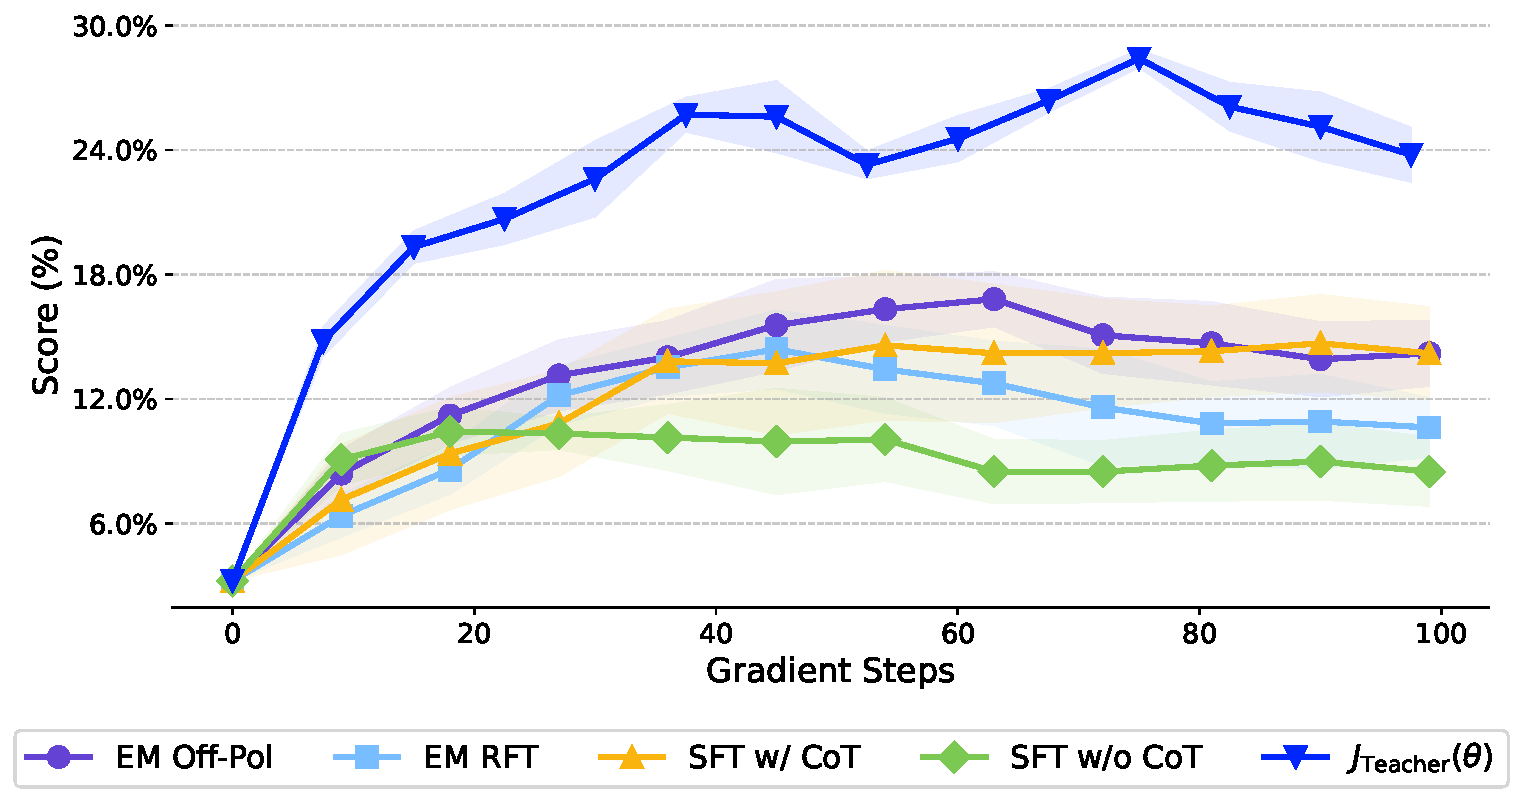
\includegraphics[width=\linewidth]{figures/sft_plot.pdf}
%         \caption{Caption}
%         \label{fig:motivation-curves}
%     \end{minipage}\hfill
% \end{figure*}


% \section{Objective Details}
% Overall from App.~\ref{app:variation-em} we obtained two tractable objectives for training:
% \begin{align}
%     \mathcal{J}_{\text{ELBO}}(\phi) &= \mathbb{E}_{(\tau,\mathbf{z}) \sim \pi^h_\phi(\cdot \mid x,h)} \left[ R(\tau,x) + \beta \log \pi_{\text{ref}}(\tau \mid \mathbf{z},x) - \beta D_{\text{KL}} (\pi^h_\phi(\mathbf{z}\mid \tau,x,h) \parallel \pi_{\text{ref}}(\mathbf{z}\mid x)) \right], \\
%     \mathcal{J}_{\text{GRPO}}(\theta) &= \mathbb{E}_{(\tau, \mathbf{z}) \sim \pi^h_\phi} \left[ \min\left( \rho_t(\theta) \hat{A}_t, \text{clip}(\rho_t(\theta), 1-\epsilon, 1+\epsilon) \hat{A}_t \right) \right].
% \end{align}
% Here we lay out precisely how we use these objectives for the different configurations presented in the main paper.


% \begin{algorithm}[t]
% \caption{$\pi$\text{-distill: Learning to Reason with Privileged Information (HintRL)}}
% \label{alg:pi_distill}
% \begin{algorithmic}[1]
% \STATE \textbf{Input:} Dataset $\mathcal{D} = \{(x, h, y)\}$, Initial Policy $\pi_\theta$, Reference $\pi_{\text{ref}}$, $\alpha$, $\beta$, $\epsilon$, Learning rate $\eta$
% \STATE \textbf{Initialize:} $\phi \leftarrow \theta$ \COMMENT{Parameters are shared between Guide and Student}
% \WHILE{not converged}
%     \STATE Sample batch $B = \{(x_i, h_i, y_i)\}_{i=1}^N \sim \mathcal{D}$
%     \STATE \textbf{// Step 1: Guide Rollout (with Hints)}
%     \FOR{each $(x, h, y) \in B$}
%         \STATE Sample $K$ trajectories $\{\tau_1, \dots, \tau_K\} \sim \pi_\theta(\cdot \mid x, h)$
%         \STATE Compute rewards $R(\tau_k) = R_{\text{env}}(\tau_k, y) - \beta \log \frac{\pi_\theta(\tau_k \mid x, h)}{\pi_{\text{ref}}(\tau_k \mid x, h)}$
%     \ENDFOR
    
%     \STATE \textbf{// Step 2: Compute Advantages (GRPO)}
%     \FOR{each $k \in \{1, \dots, K\}$}
%         \STATE $A_k = \frac{R(\tau_k) - \text{mean}(\{R(\tau_j)\}_j)}{\text{std}(\{R(\tau_j)\}_j) + \delta}$
%     \ENDFOR
    
%     \STATE \textbf{// Step 3: Compute Objectives}
%     \STATE \textbf{Guide Loss (ELBO):} 
%     \STATE $\mathcal{L}_{\text{Guide}} = -\frac{1}{K} \sum_{k=1}^K \log \pi_\theta(\tau_k \mid x, h) \cdot A_k$
    
%     \STATE \textbf{Student Loss (Off-Policy GRPO):}
%     \STATE Compute IS weights: $\rho_k = \frac{\pi_\theta(\tau_k \mid x)}{\pi_\theta(\tau_k \mid x, h)}$ \COMMENT{Note: Student input is $x$ only}
%     \STATE $\mathcal{L}_{\text{Student}} = -\frac{1}{K} \sum_{k=1}^K \min \left( \rho_k A_k, \text{clip}(\rho_k, 1-\epsilon, 1+\epsilon) A_k \right)$
    
%     \STATE \textbf{// Step 4: Joint Update}
%     \STATE $\mathcal{L}_{\text{Total}} = \alpha \mathcal{L}_{\text{Guide}} + (1 - \alpha) \mathcal{L}_{\text{Student}}$
%     \STATE $\theta \leftarrow \theta - \eta \nabla_\theta \mathcal{L}_{\text{Total}}$
% \ENDWHILE
% \end{algorithmic}
% \end{algorithm}








\newpage
\section{Additional Ablations}
\label{app:leakage_ablation}
\subsection{Privilege Information leakage Ablation}
We measure privileged-information leakage with a simple keyword detector applied to each assistant message, using the keyword list [``privileged information'', ``privileged info'', ``priv info'', ``secret information'', ``secret info'', ``correct tool calls'', ``secret'', ``privileged'', ``hint'', ``hints'']. For each occurrence, we assign a penalty of $-0.1$ and accumulate it over the trajectory, and we mark a trajectory as leaking if any of these appear. Fig \ref{fig:priv-info-curves} reports results at $\beta = 0.25$ and shows that enabling this leakage penalty does not change task performance in any noticeable way, since the learning curves with and without the penalty overlap closely. Fig \ref{fig:keywork-analysis} shows the corresponding leakage rate during training, and it rises as training progresses across all modes. The pattern with tool-calls showing the highest leakage, tool calls and arguments increasing more moderately, and self-generated hints starting lower but still increasing over time.


% \EP{Describe information leakage say it doesnt do anything show that the information leakage risees as training goes on regardless seems to be hint specifc}

\begin{figure}[H]
\centering
    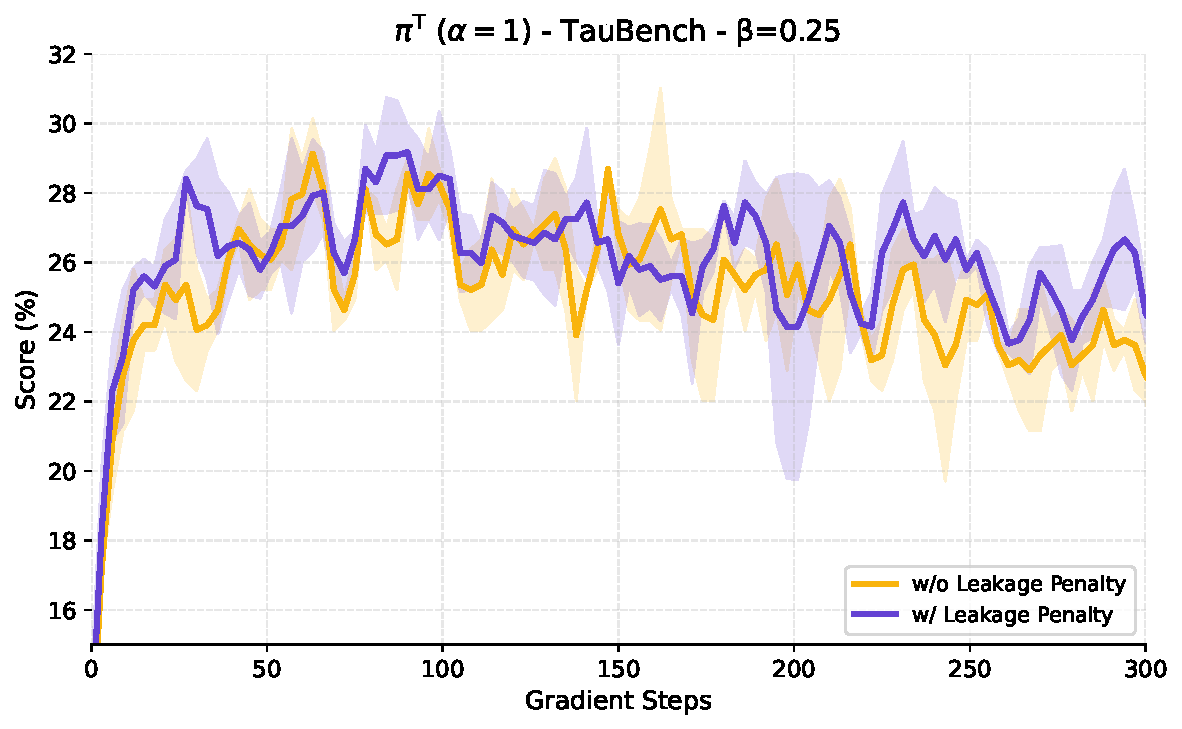
\includegraphics[width=0.65\linewidth]{figures/leakage_penalty_comparison.pdf}
    \caption{Performance with and without leakage penalty for $\pi^{\text{T}} (\alpha=1)$. We find that although the penalty does reduce the leakage of the privileged information (see \Cref{fig:keywork-analysis}) it does not affect performance.}
    \label{fig:priv-info-curves}
\end{figure}


\begin{figure}[H]
\centering
    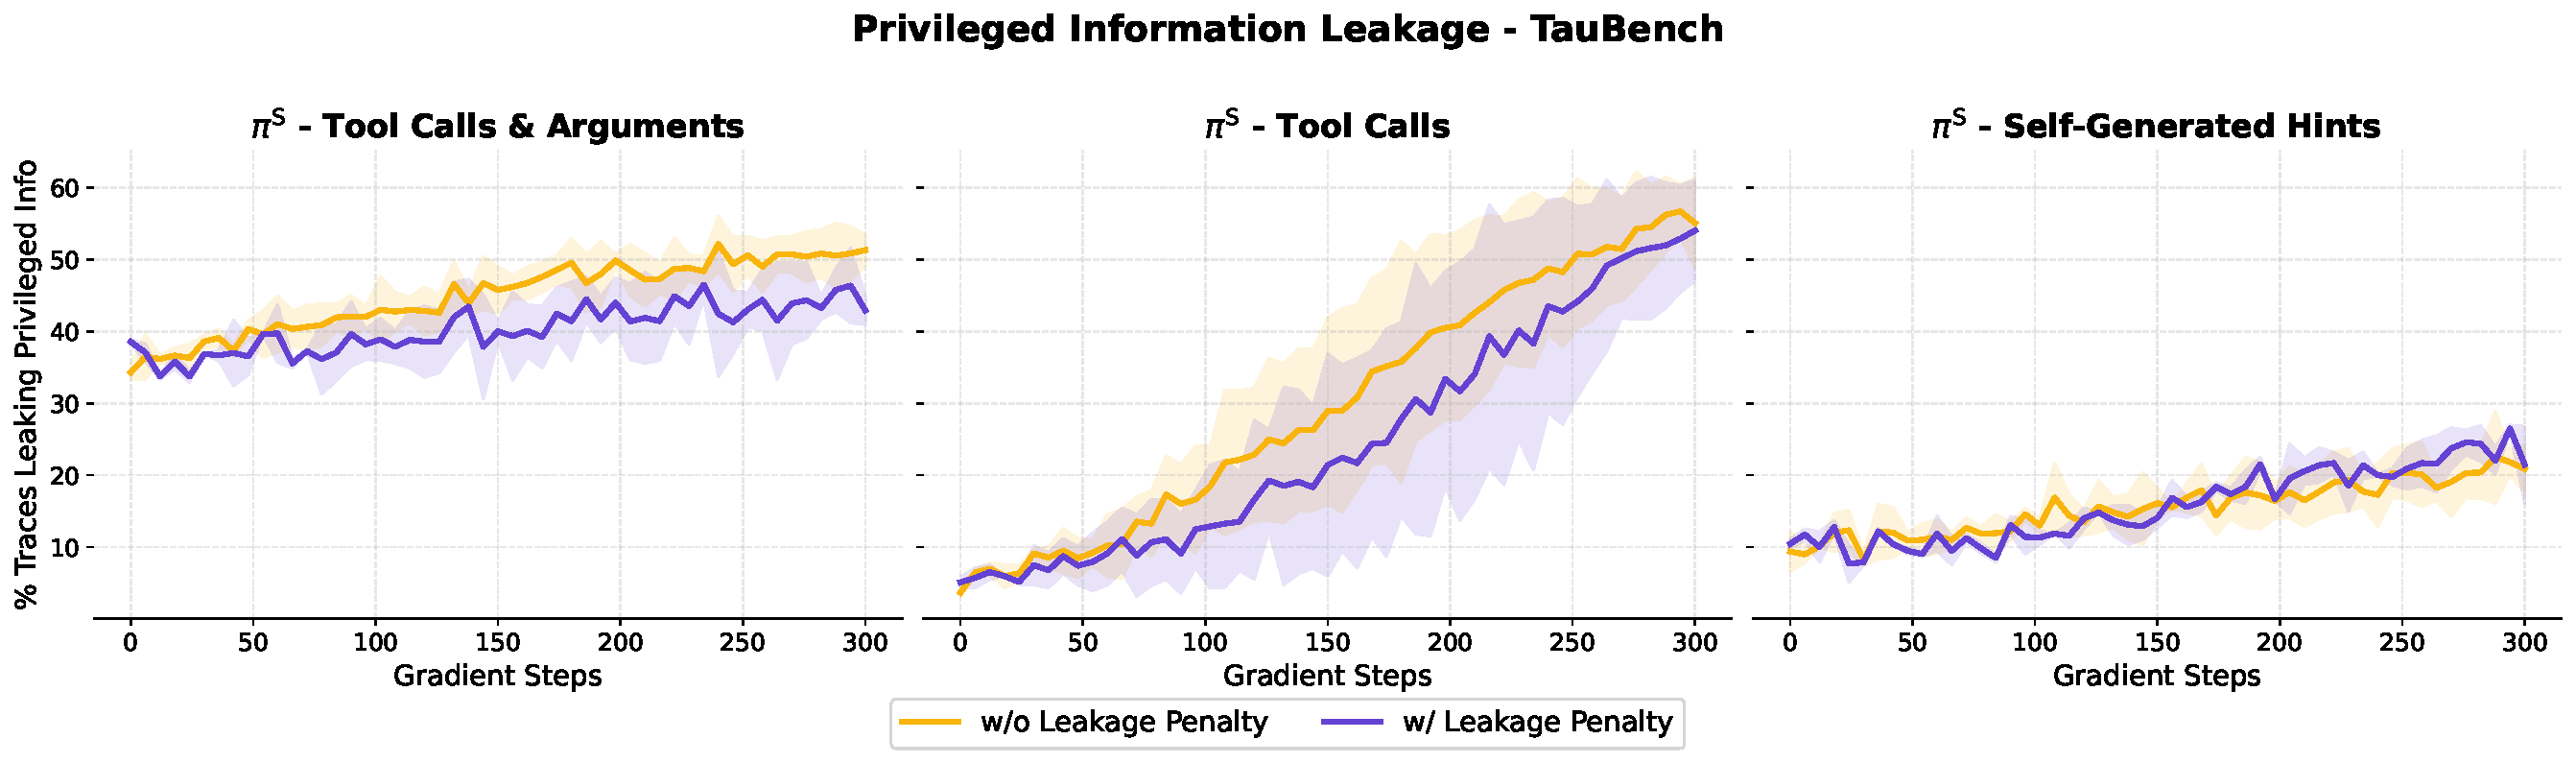
\includegraphics[width=0.95\linewidth]{figures/leakage_keyword_analysis_all.pdf}
    \caption{Proportion of traces leaking privileged information as training progresses, we see that regardless PI type, the leakage increases with more gradient steps, finding using a leakage penalty reduces this proportion, but not substantially. }
    \label{fig:keywork-analysis}
\end{figure}


\paragraph{Test-time leakage.} As an additional analysis, we analyze whether leakage increases as models are trained with privileged data when evaluating $\piS$. \Cref{fig:eval-keywork-analysis} outlines this for \texttt{Qwen3-8B} for 300 gradient steps. We empirically validate that leakage does not significantly affect or increase when evaluating using $\piS$ as the presence of leaked words does not meaningfully increase as training continues.
\begin{figure}[H]
\centering
    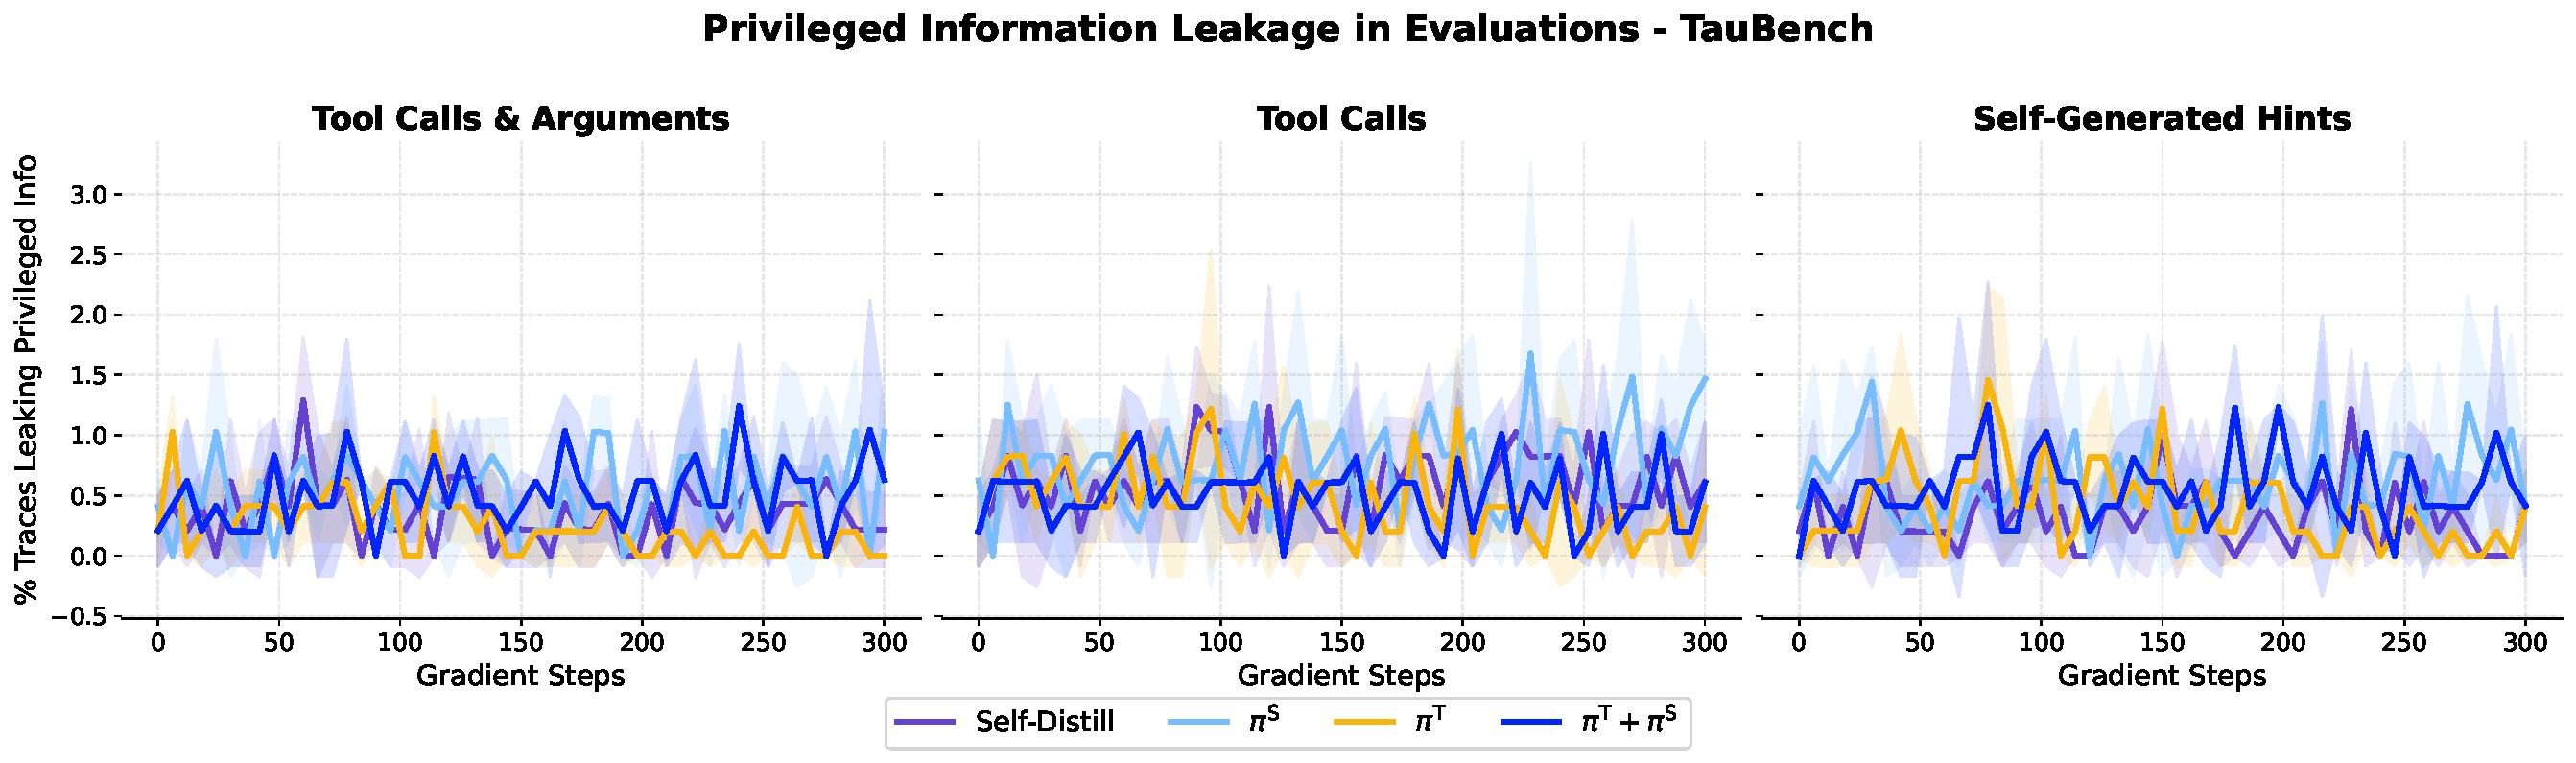
\includegraphics[width=0.95\linewidth]{figures/leakage_algo_comparison_evals.pdf}
    \caption{Proportion of traces leaking privileged information when \textbf{evaluating} $\piS$ as training progresses, we see that there is no increase in leakage when evaluated as training goes on.  }
    \label{fig:eval-keywork-analysis}
\end{figure}


\subsection{Reference Model Ablation}

\label{app:ref-model-ablation}
We ablate the choice of reference policy used in the KL term by comparing a fixed base reference, $\pi_{\text{base}}$, against using the student itself as the reference, $\pi_\theta$ (with stop-gradient on the reference branch). Fig.\ref{fig:placeholder_5} shows a clear difference in training stability. When $\pi_{\text{base}}$ is used as the reference, the performance degrades over training and can collapse most clearly in the $\pi^h$ setting ($\alpha=1$), where the policy is pushed to move far from the base while still being penalized for that same deviation. In contrast, using $\pi_\theta$ as the reference (orange) yields stable learning across $\alpha \in \{0, 0.5, 1\}$, since the KL regularizer stays aligned with the current student distribution. Practically, this choice is also cheaper because using $\pi_\theta$ as the reference avoids maintaining a separate frozen reference model on the GPU, reducing memory and compute overhead.


\begin{figure}[h!]
    \centering
    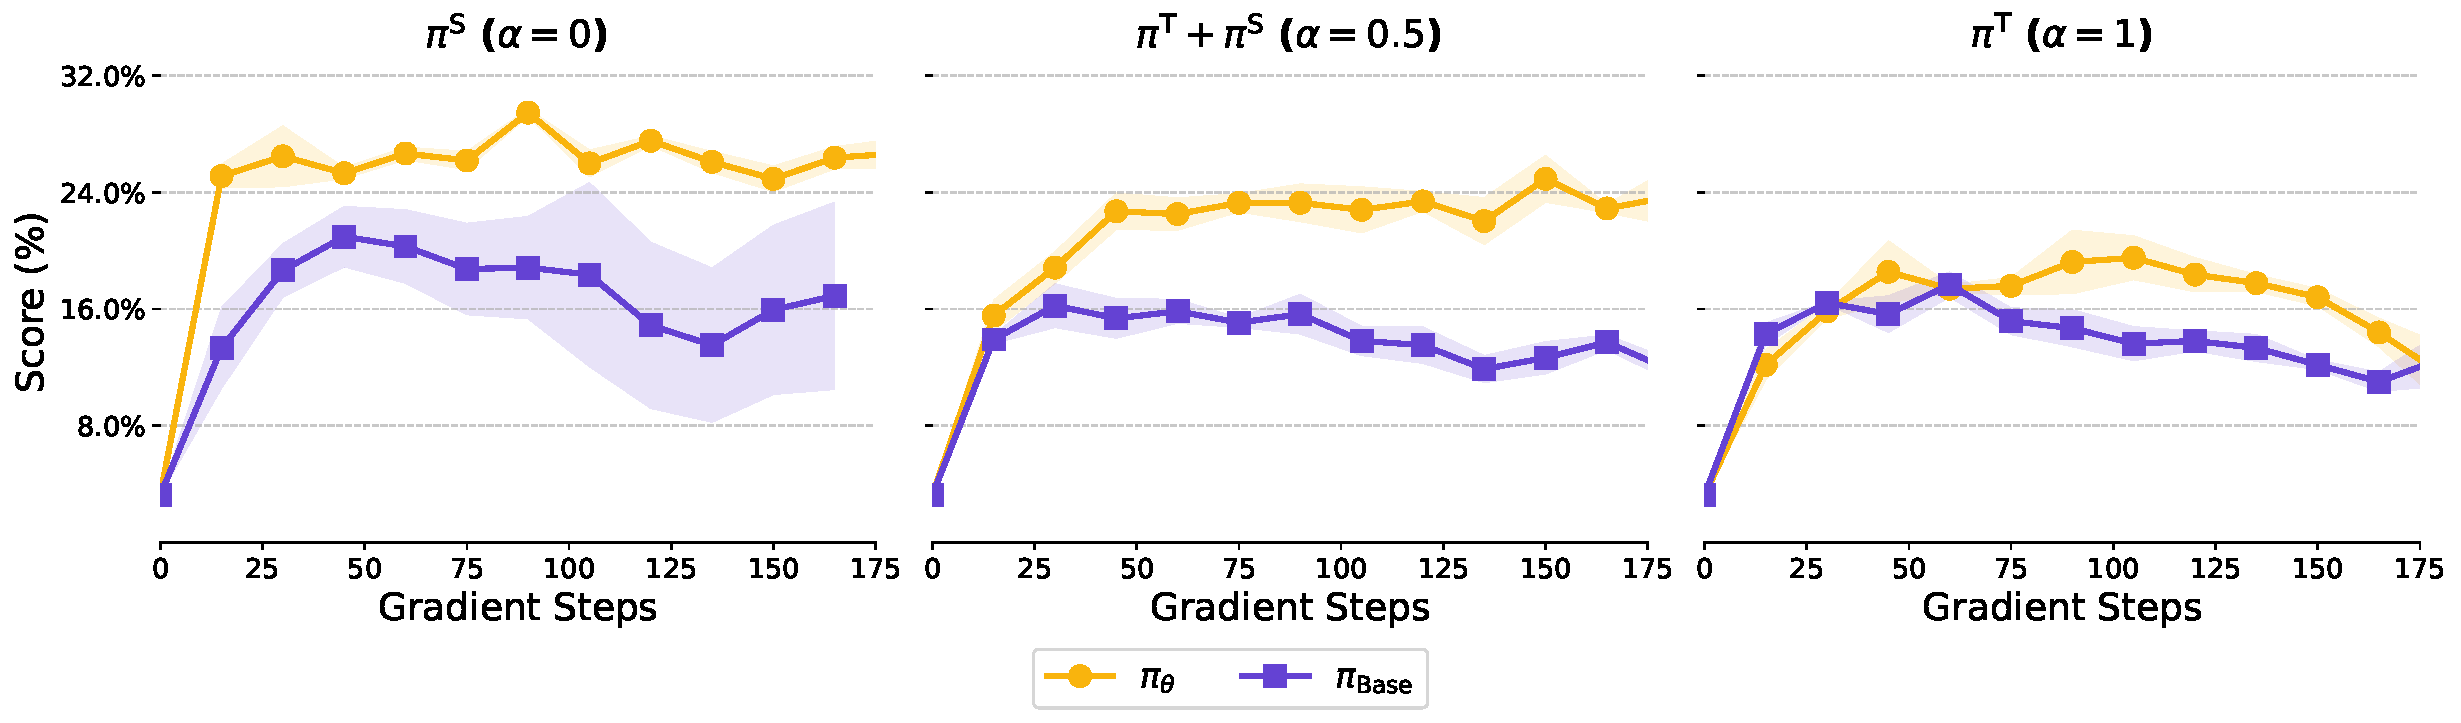
\includegraphics[width=1\linewidth]{figures/hp_comparison_update_ckpt.pdf}
    \caption{Ablation between using reverse-Kl between the teacher and a prior. We ablate over two possible priors, $\pi_{\text{base}}$ and $\pi^\text{S}_\theta$. We find that using  $\pi^\text{S}_\theta$ to be highly important in obtaining best performance.}
    \label{fig:placeholder_5}
\end{figure}
\newpage

\subsection{Full $\beta$ Ablations}
\Cref{fig:beta-full} outlines the full suite of $\beta$ ablations for $\pi$-Distill variants and self-distillation for \texttt{Qwen3-4/8B}. We sweep over $\beta \in \{0.1,0.25,0.5 \}$.


\begin{figure}[H]
    \centering
    % Top Figure
    \begin{minipage}{\linewidth}
        \centering
        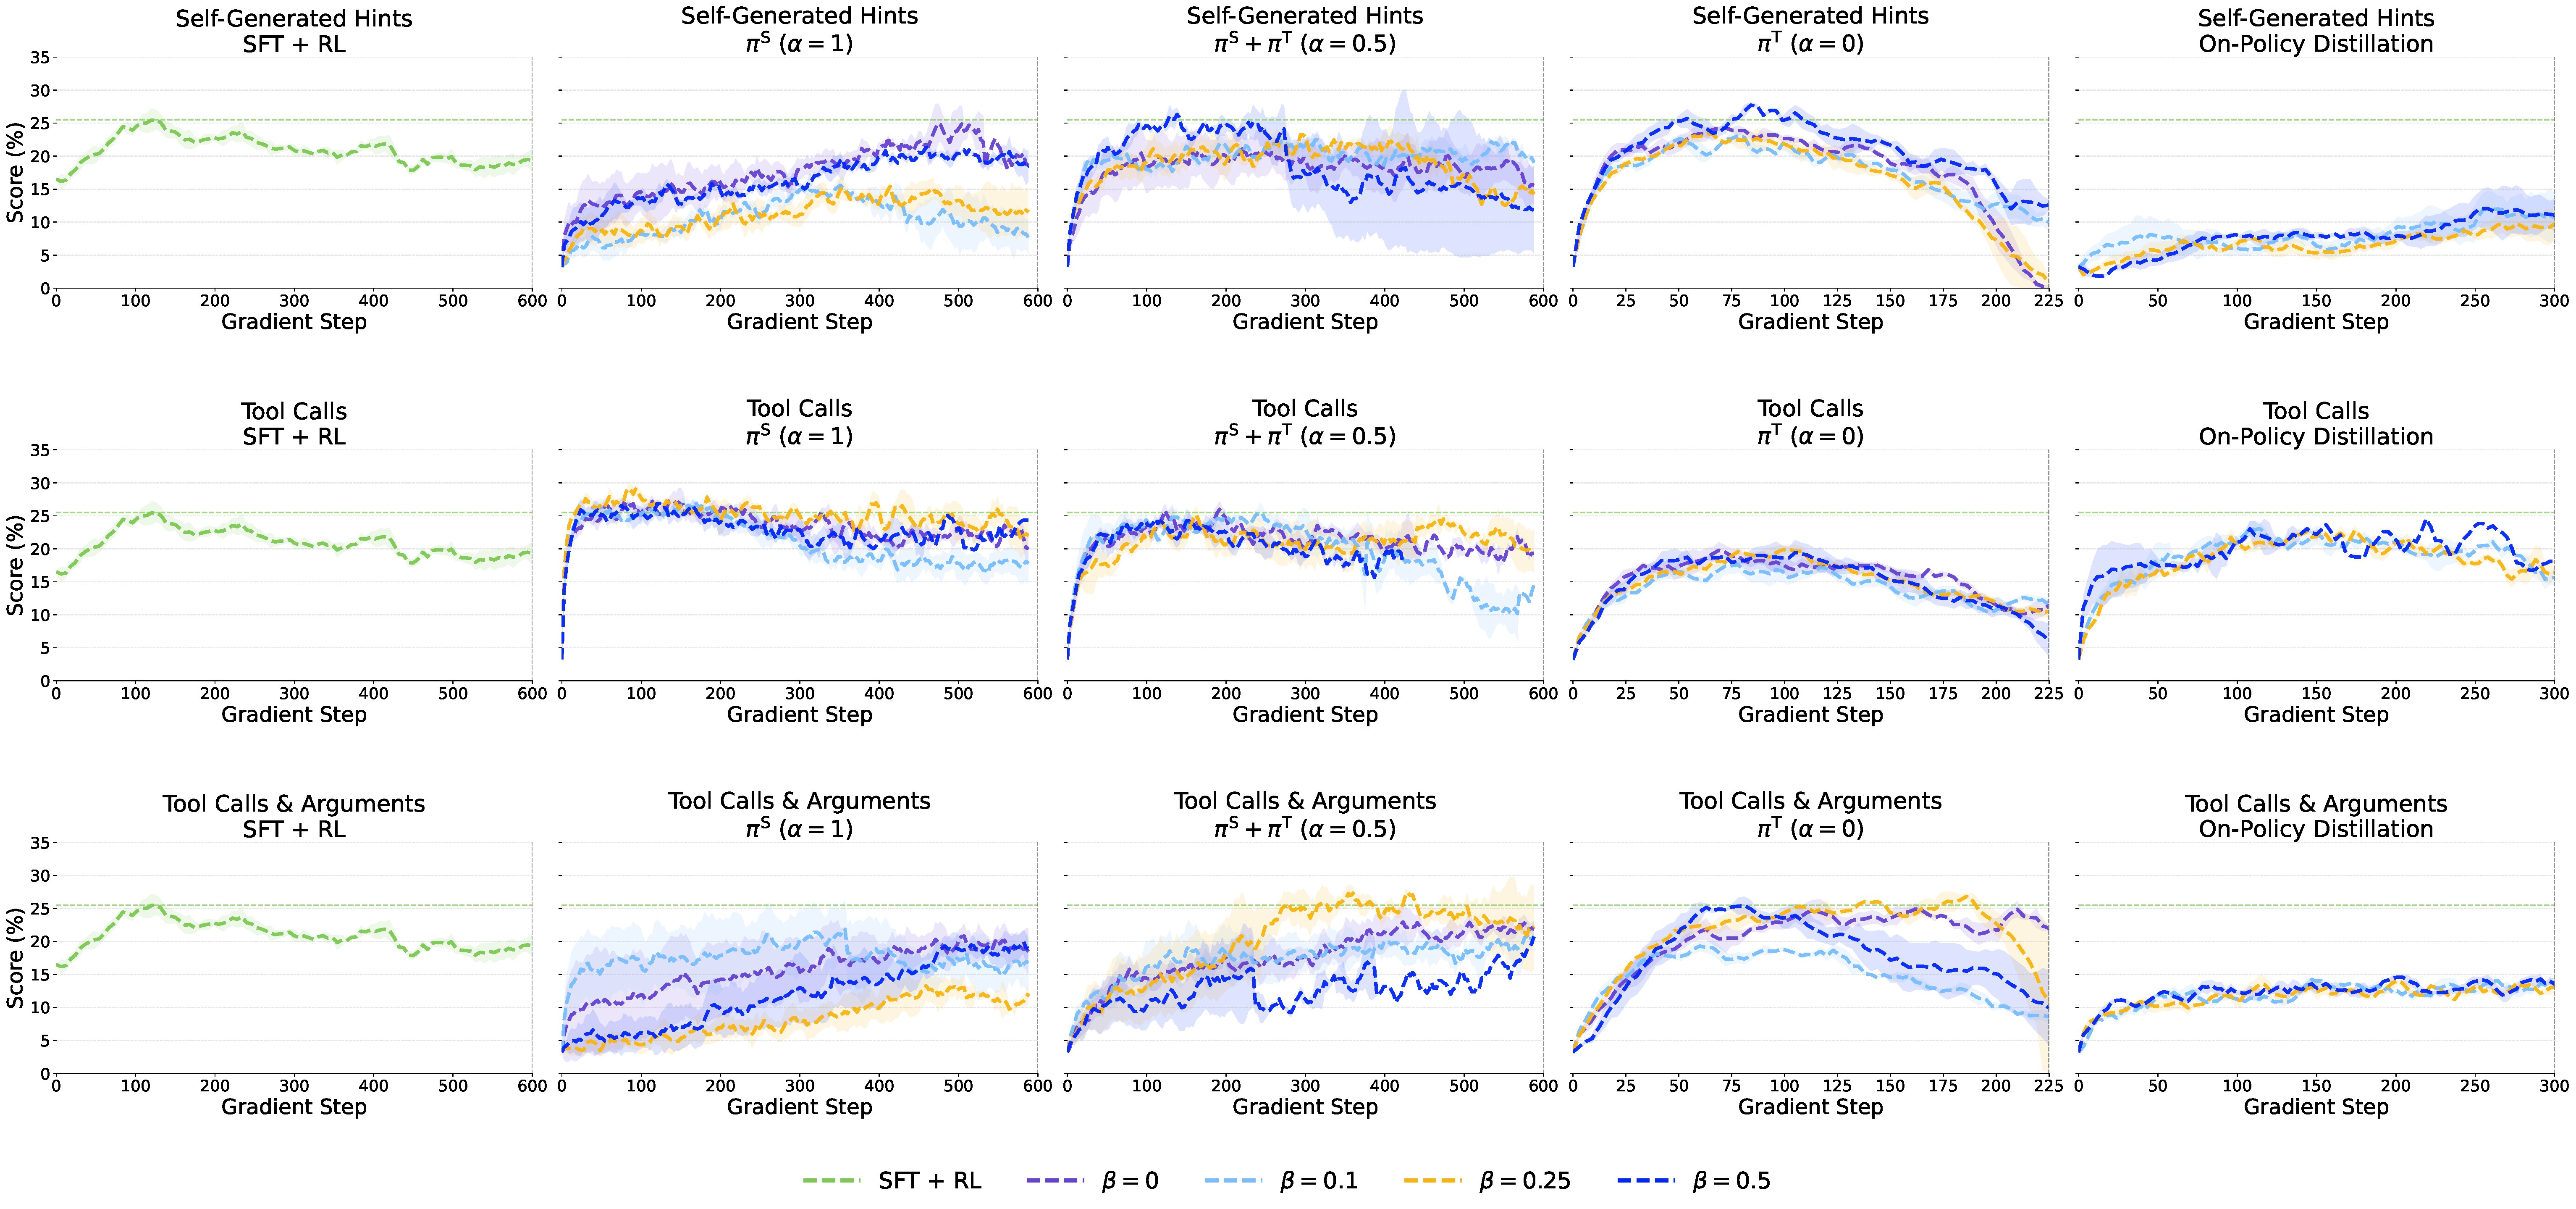
\includegraphics[width=\linewidth]{figures/beta_grid_qwen3_8b_taubench.pdf}
        \centerline{(a) \texttt{Qwen3-8B}}
    \end{minipage}
    
    \vspace{0.5cm} % Space between them

    % Bottom Figure
    \begin{minipage}{\linewidth}
        \centering
        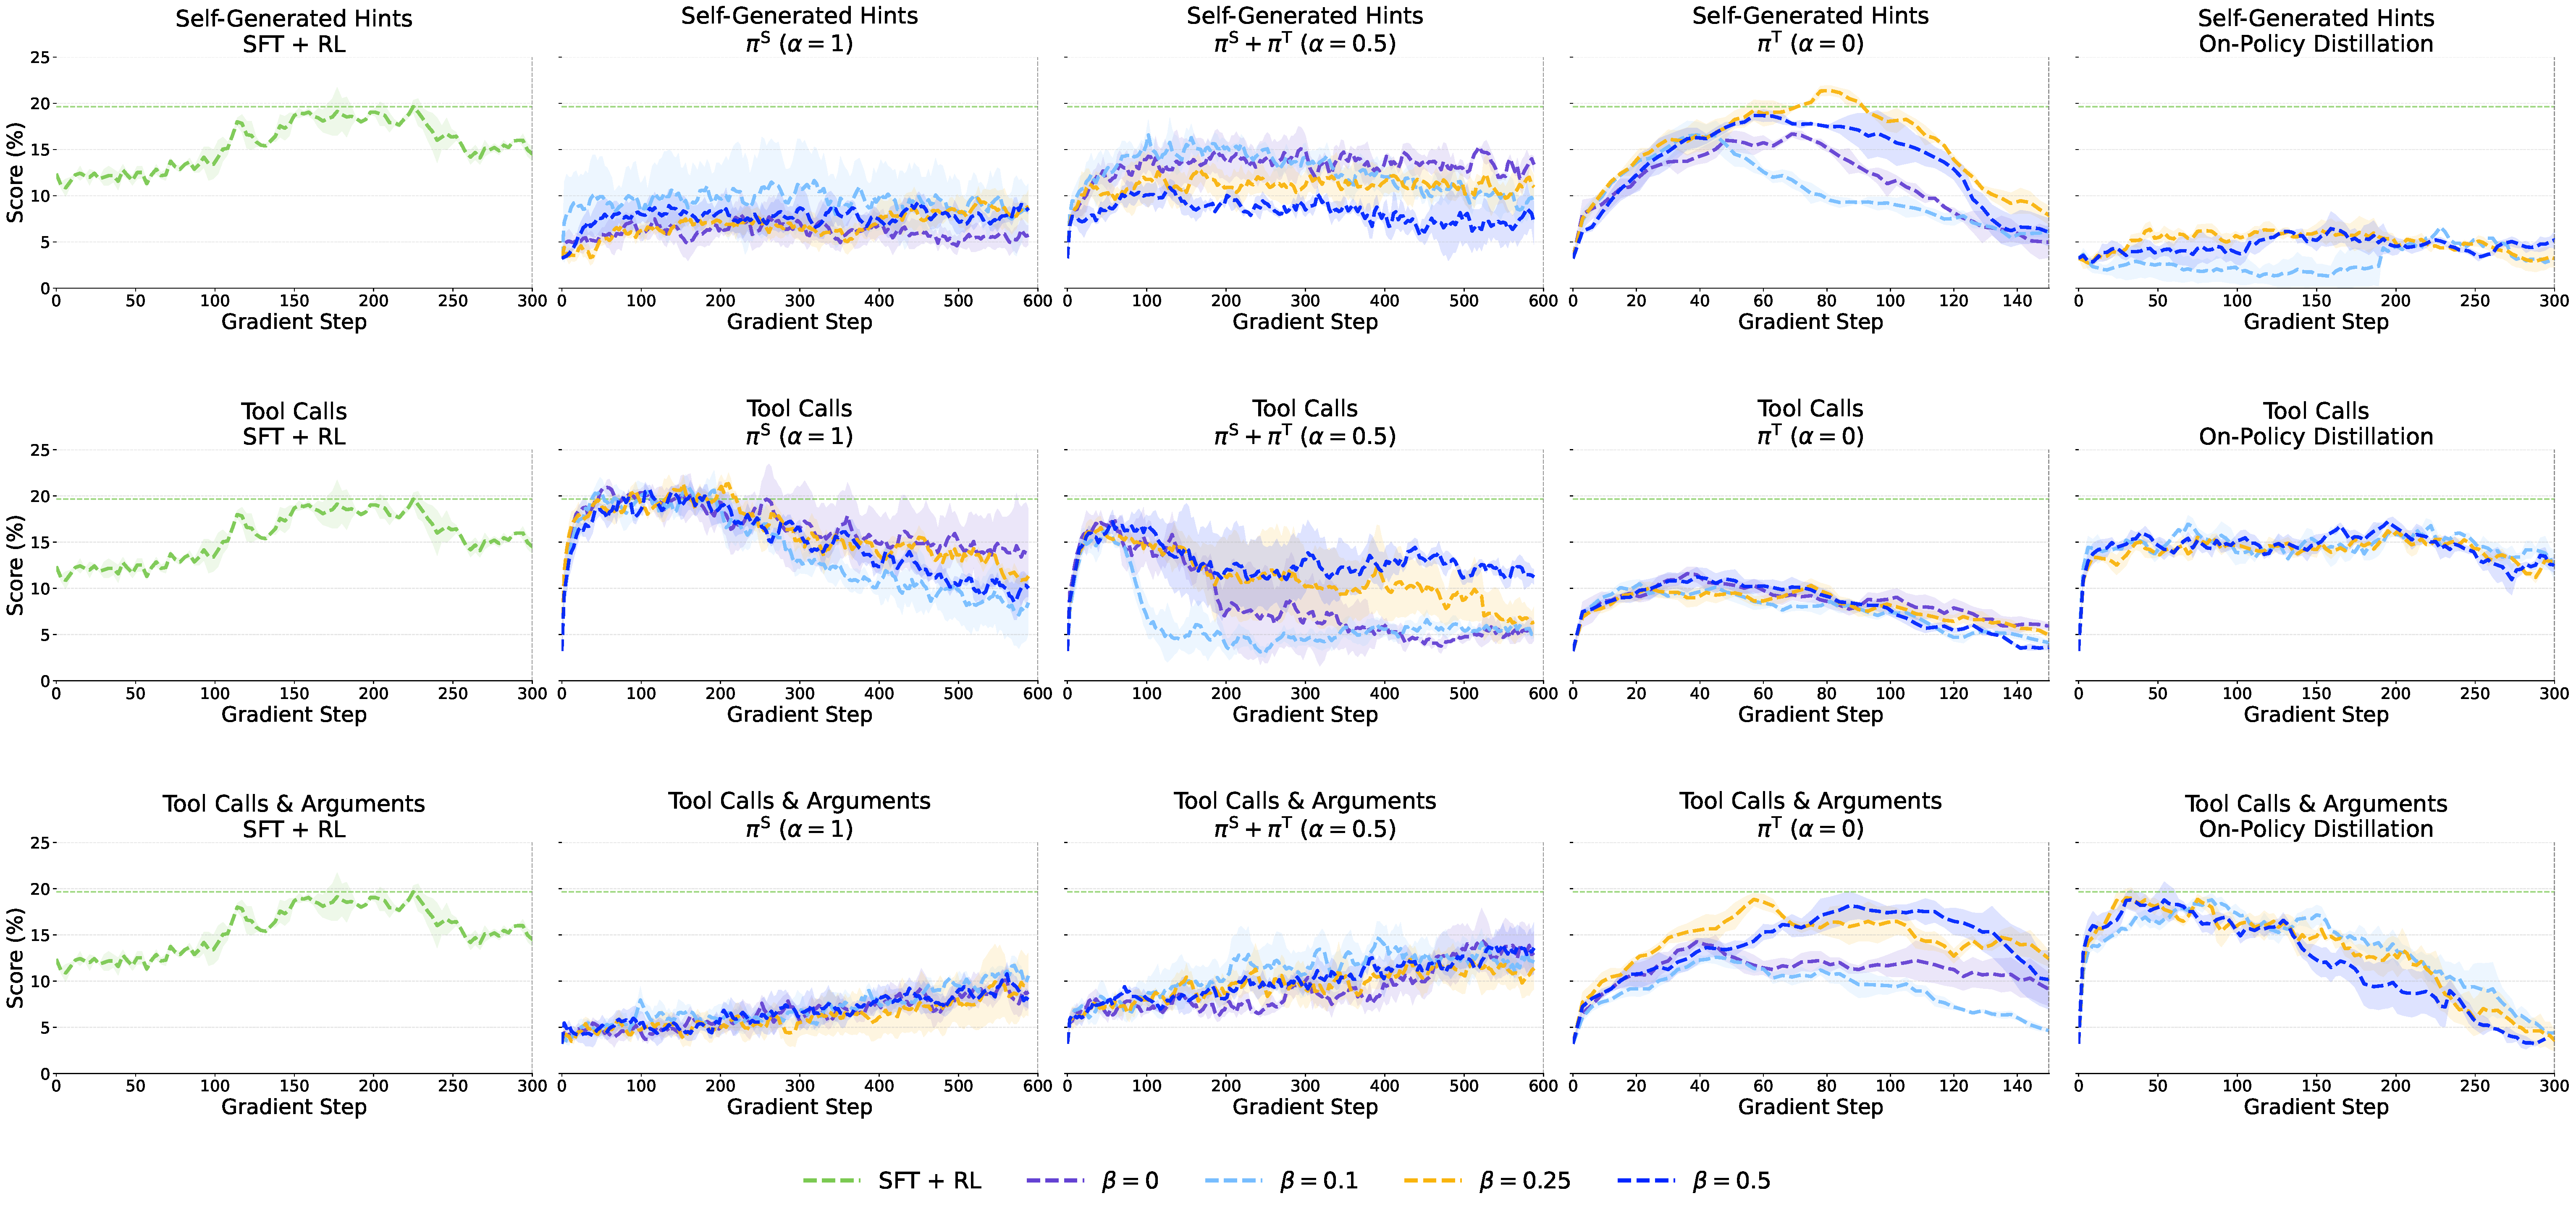
\includegraphics[width=\linewidth]{figures/beta_grid_qwen3_4b_taubench.pdf}
        \centerline{(b)\texttt{Qwen3-4B}}
    \end{minipage}

    \caption{Full sweep for $\beta$ over variants of $\pi$-Distill. All experiments are given a 600 gradient step budget, where here we cut off experiment types early if they crash or do not continue learning. Consistent performance gains are seen for $\beta > 0$ across both 8B and 4B scales. We find that $\beta>0$ is important in 14/18 cases. Specifically, we find it most important when training $\piT$ and less important with student-only training $\piS$. }
    \label{fig:beta-full}
\end{figure}
\newpage
% Caption suggestion for Fig. 7:
% \caption{Reference model ablation for the KL term on TauBench. We compare using a fixed base reference $\pi_{\text{base}}$ versus using the student as the reference $\pi_\theta$ (stop-gradient). Using $\pi_{\text{base}}$ can destabilize training and cause performance collapse, especially for $\alpha=1$, while $\pi_\theta$ yields stable performance and avoids the need to load a second reference model.}


\section{Implementation setup - Further details}

\label{app:imp-details}
\subsection{KL Estimator}

For all losses requiring a Kl estimation, we use the Rae-Blackwellized estimator\citep{amini2025betterestimationkullbackleiblerdivergence}. For $\pi$-Distill, we use a sequence-level penalty aggregated into the reward term  
following \citet{shah2026comedyestimatorsklregularization}. In this setting, we allow the KL penalty to be absorbed into the advantage computation. 

For OPSD, we use the same estimator as in \citep{amini2025betterestimationkullbackleiblerdivergence} and directly back-propagate through the estimation. 

\subsection{Length Penalty}
\label{app:length-penalty}
In our setting, we found that policies can become overly verbose. To mitigate this, we add a cosine-shaped length penalty inspired by the cosine length-scaling reward \cite{yeo2025demystifyinglongchainofthoughtreasoning}. We apply this penalty only to successful traces (i.e., when the base reward $r>0$). For each assistant turn $i$ with token length $l_i$, we use a no-penalty threshold $l_{\text{th}}=2000$ and a soft allowance $l_{\max}=5000$. If $l_i \le l_{\text{th}}$, the turn penalty is $p_i=0$ otherwise we assign a negative penalty using a linear--cosine schedule that increases in magnitude with length, approaching $-\lambda$ near $l_{\max}$ with $\lambda=0.1$, and becoming harsher beyond $l_{\max}$ (up to an endpoint of $-2\lambda$). We then average the per-turn penalties across the $N$ assistant turns:
\[
\bar{p} = \frac{1}{N}\sum_{i=1}^{N} p_i .
\]
We cap the total penalty as $p_{\text{total}}=\max(\bar{p},-0.3)$ and add that to the base reward $r'=r+p_{\text{total}}$.



% \subsection{Hyperparameter Choices}
% \label{app:hyperparams}

% \textbf{Seeds:} 3. \\
% \textbf{Rollout temperature:} 0.75. \\
% \textbf{Trace length filter:} discard traces if tokens are above 25k for TauBench and for TravelPlanner RL, 35k tokens are allowed \\
% \textbf{Advantage processing:} pop zero-advantage is always used \\

% \textbf{Training budgets:}
% TauBench total gradient steps = 600; TravelPlanner total gradient steps = 400. \\
% \textbf{Updates per sampling phase:}
% TauBench = 3; TravelPlanner = 2. \\

% \textbf{Repeats per group:}
% TauBench = 5; TravelPlanner = 4. \\
% % \textbf{All-tasks TravelPlanner:} \EP{(fill in if you have a specific flag/value)} \\

% \textbf{Repeat budget for training sets:}
% TauBench $\pi$-distill = 64; SFT+RL = 128. \\

% \textbf{Learning-rate sweep:} $\{1\mathrm{e}{-}6,\; 5\mathrm{e}{-}6,\; 1\mathrm{e}{-}5\}$. \\
% \textbf{Final LR choices:}
% TauBench = $5\mathrm{e}{-}6$; TravelPlanner $\pi$-distill = $1\mathrm{e}{-}5$; TravelPlanner RL = $5\mathrm{e}{-}6$. \\

% \textbf{Clipping / epsilon:}
% standard lower = 0.8 and upper = 1.2. \\
% upper sweep = $\{1.0,\;1.2,\;1.5\}$; no differences observed $\Rightarrow$ use upper = 1.2. \\
% applied to student + teacher losses and all RL. \\

% \textbf{$\alpha$ annealing (important):}
% for $\alpha=0.5$, linearly anneal $\alpha: 0 \rightarrow 0.5$ over 15 epochs to prevent early collapse between $p$ and $q$. \\

% \textbf{Context parallelism:}
% TravelPlanner contexts are long, so we use context parallelism (slower training). \\

\subsection{Hyper-Parameters}

Here \cref{tab:hyperparams_models} we outline the swept hyperparameters, as well as their final values. 
\label{app:hps}
\begin{table}[h]
\centering
\footnotesize
\setlength{\tabcolsep}{4pt}
\begin{tabular}{@{}lp{4.5cm}ccc@{}}
\toprule
\textbf{Category} & \textbf{Parameter} & \textbf{R1-Distill-Llama-8B} & \textbf{QWEN3-4B} & \textbf{QWEN3-8B} \\
\midrule
\multirow{4}{*}{\textbf{General}} 
& Seeds & 3 & 3 & 3 \\
& Rollout temperature & 0.75 & 0.75 & 0.75 \\
& Trace length filter & \multicolumn{3}{c}{Discard if tokens $>$ 25k ($\tau$-Bench/TP), $>$ 35k (RL/OPSD)} \\
& Advantage processing & \multicolumn{3}{c}{pop zero-advantage (always)} \\
\midrule
\multirow{2}{*}{\textbf{Training Budgets}} 
& $\tau$-Bench total gradient steps & 600 & 600 & 600 \\
& TP total gradient steps & 400 & 400 & 400 \\
\midrule
\multirow{3}{*}{\textbf{Sampling}} 
& Gradient steps per sampling & \multicolumn{3}{c}{$\tau$-Bench = 3, TP = 2} \\
& Repeats per group & \multicolumn{3}{c}{$\tau$-Bench = 5, TP = 4} \\
& Training tasks sampled & \multicolumn{3}{c}{$\tau$-Bench = 64, TP = 45, SFT+RL ($\tau$-Bench) = 128} \\
\midrule
\multirow{4}{*}{\textbf{Optimization}} 
& Learning-rate sweep & \multicolumn{3}{c}{\{1e{-}6, 5e{-}6, 1e{-}5\}} \\
& Final LR & \multicolumn{3}{c}{$\tau$-Bench: 5e{-}6 for all, TP: $\pi$-distill = 1e{-}5, RL/OPSD = 5e{-}6} \\
& $\beta$ & \multicolumn{3}{c}{TP/OPSD = 0.5, $\pi$-distill = 0.25 (unless swept)} \\
& Clipping/epsilon & \multicolumn{3}{c}{Lower = 0.8, Upper = 1.2} \\
\midrule
\textbf{Alpha Annealing} 
& $\alpha=0.5$ schedule & \multicolumn{3}{c}{Linearly anneal $\alpha: 0 \rightarrow 0.5$ over 15 epochs} \\
\bottomrule
\end{tabular}
\caption{Hyperparameters used for each fine-tuned model. All models share identical hyperparameter settings. Travel Planner is abbreviated to TP.}
\label{tab:hyperparams_models}
\end{table}






% \section{Prompt}

% \section{Additional Analysis on Privileged Information}


\section{Plot and Table Discrepancies}
% \EP{write things for this on the discrepancy between averaging seeds and the runs} 
In this Fig \ref{fig:plot-table-discreptancies}, the 31.11\% number is computed from the three seed peaks in the right panel. Each seed reaches its best score at a different gradient step, roughly one around 70 steps, another around 95, and another around 150. We take those three peak values and average them, which gives 31.11\%, and that is what is reported in the table. The left panel instead shows the mean score at each gradient step, averaging the seeds at the same step, so its peak corresponds to the best point of the averaged curve rather than the average of the three best points. This difference in aggregation means the table can be higher than the peak of the averaged curve shown in the left plot.

\label{app:example-discreptency}
\begin{figure}[h!]
    \centering
    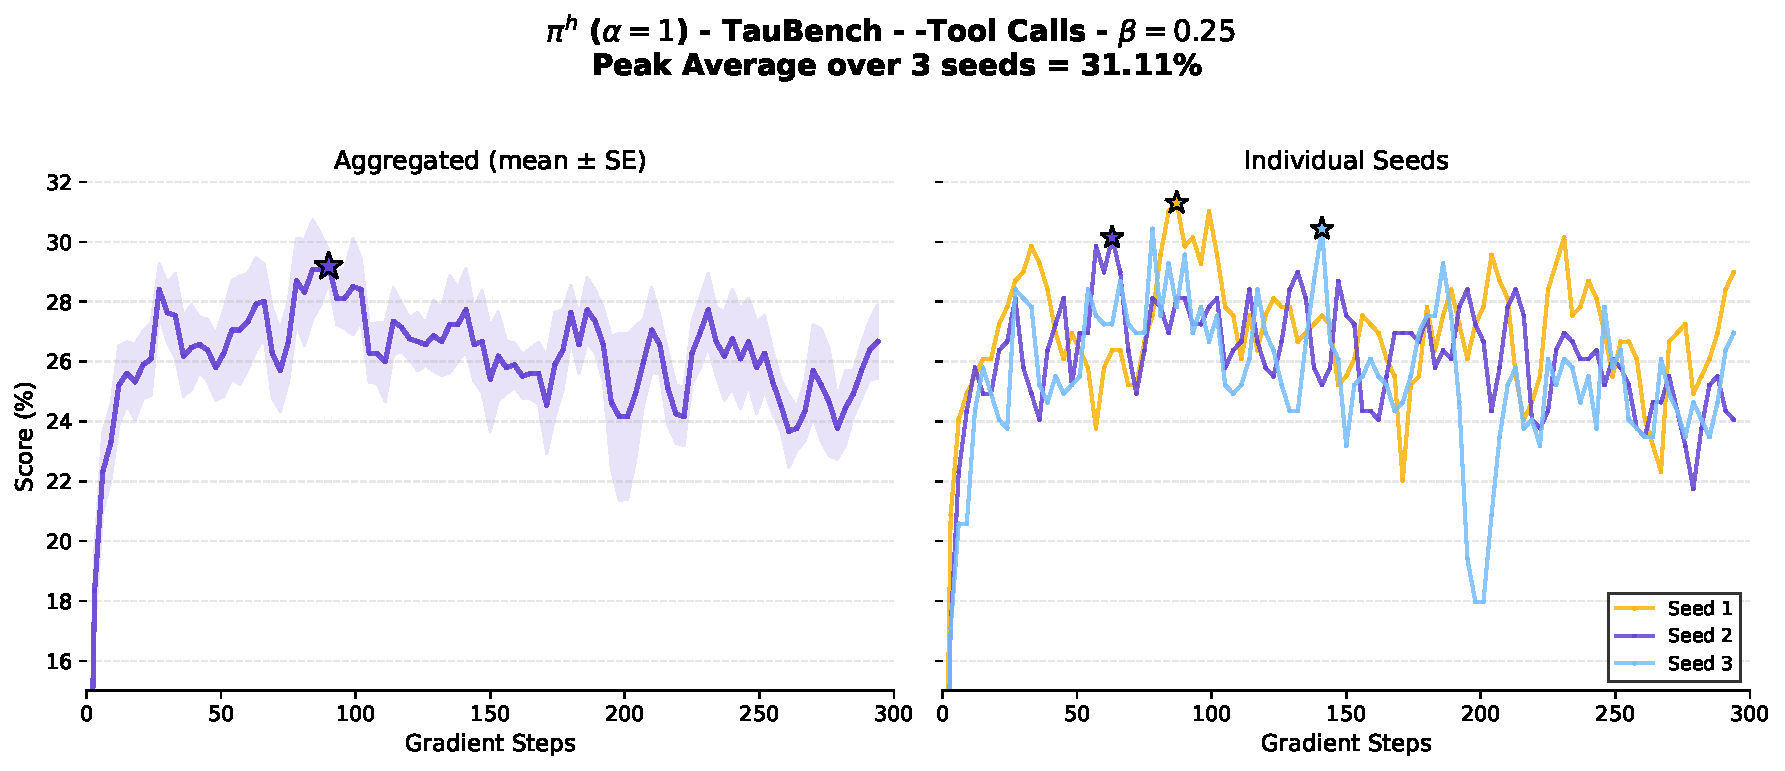
\includegraphics[width=0.85\linewidth]{figures/three-seed-plot.pdf}
    \caption{Comparison aggregating training runs versus the individual training runs. The left figure displays the mean score across seeds at each gradient step, while the right panel highlights the individual trajectories where peaks occur at different intervals. The reported table value ($31.11\%$) represents the average of these individual seed peaks.}
    \label{fig:plot-table-discreptancies}
\end{figure}

\section{Reward Hacking in Travel Planner}
\label{app:tp-hack}

Our early experiments show that the model is able to consistently reward-hack the original rubric-based rewards proposed by \cite{xie2024travelplannerbenchmarkrealworldplanning}. Specifically, \Cref{fig:planner_hack} shows the learning curves under the original reward structure. The policy appears to steadily improve; however, upon inspection, we observe that all traces collapse to the response structure shown in \Cref{prompt:tp-hack}. We attribute this behavior to the model learning that invoking the \texttt{Planner[.]} tool ends the conversation and, with certain arguments, reliably yields a high reward.

We address this issue by removing the requirement that all “easy” constraints must be satisfied before any “hard” constraint is checked. Instead, we evaluate each easy constraint individually and, only if it is satisfied, we then check its corresponding hard constraint.

\begin{figure}[h!]
    \centering
    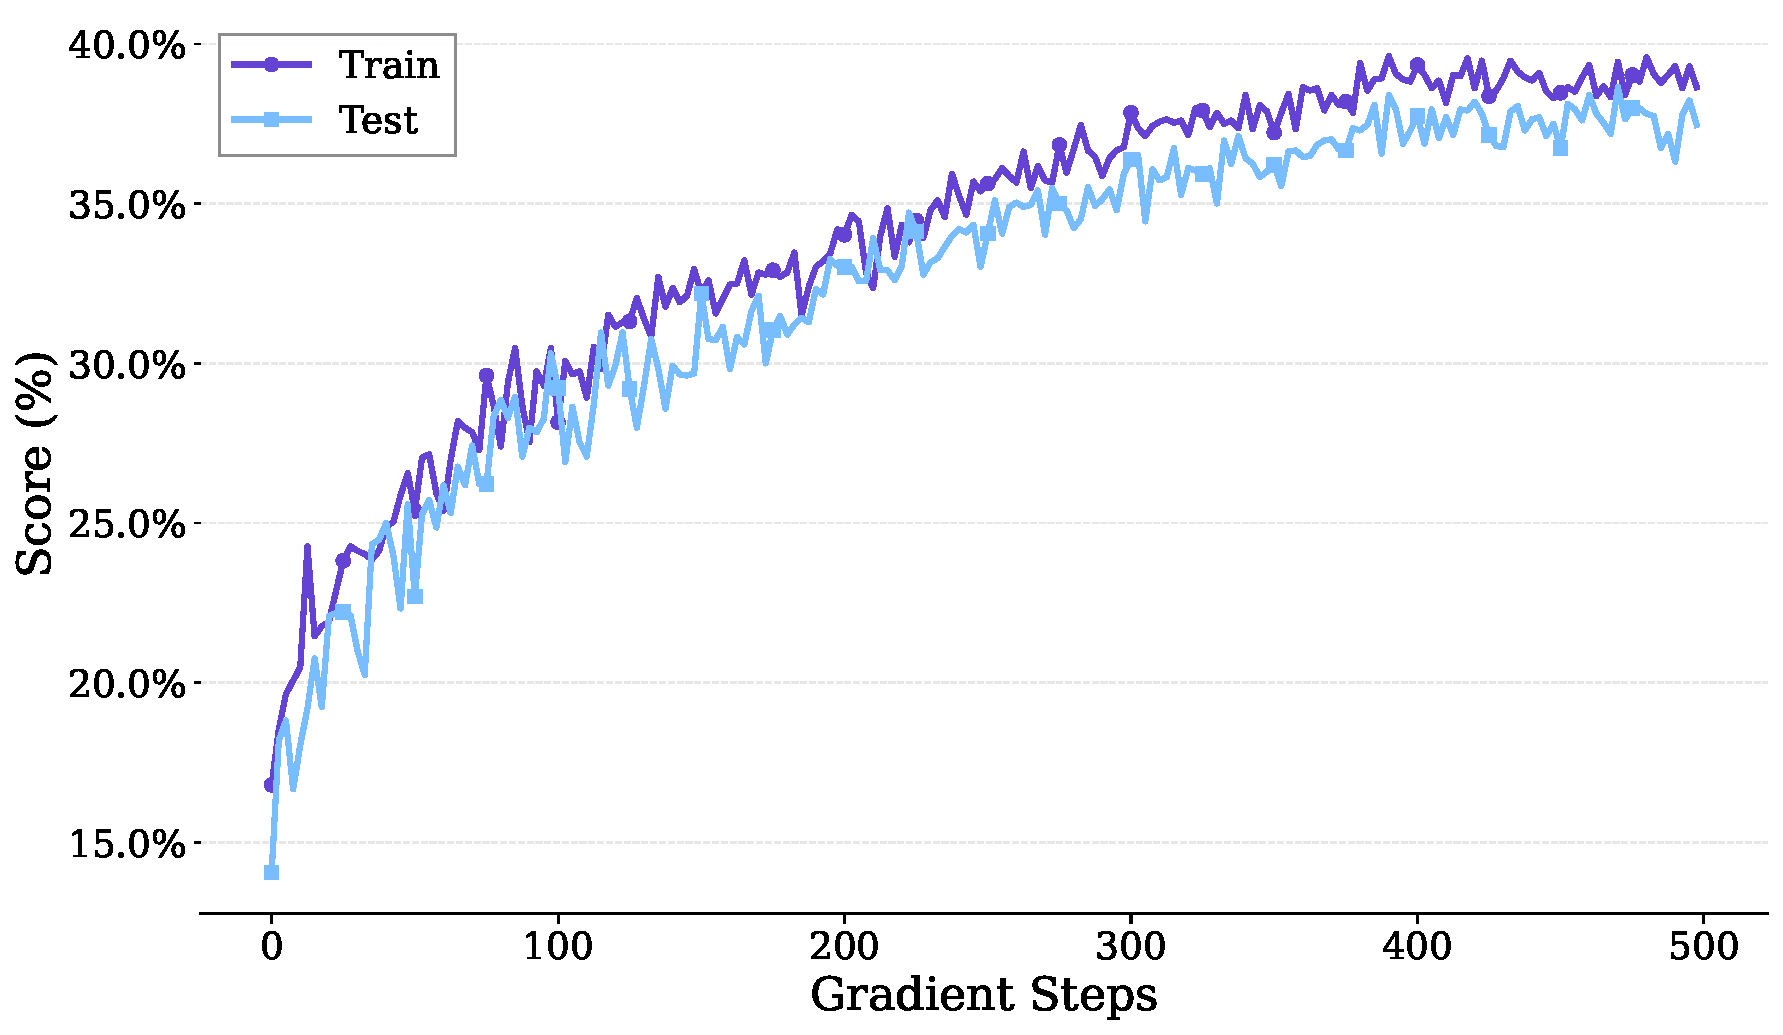
\includegraphics[width=0.75\linewidth]{figures/priv_train_q_gamma0_planner_qwen3_4b.pdf}
    \caption{Training and testing curves for Travel Planner, using the original reward structure proposed in \cite{xie2024travelplannerbenchmarkrealworldplanning} with \texttt{Qwen3-4B}. We find that while the model learns, the sequences generally converge on reward hacking. Where the entire score is dominated by the ''easy constraint score'' as the model has learnt to satisfy some basic constraints, leading to the policy outputting the same response for all queries.}
    \label{fig:planner_hack}
\end{figure}



\lstdefinestyle{promptcode}{
    basicstyle=\ttfamily\footnotesize,
    breaklines=true,
    breakatwhitespace=true,
    columns=fullflexible,
    keepspaces=true,
    showstringspaces=false,
    frame=none
}
\begin{prompt}{$\tau$-Bench Travel Planner Model Trajectory}
\label{prompt:tp-hack}
\textbf{Role:} Assistant  

\begin{lstlisting}[style=promptcode]
<think>
Okay, let's tackle this travel planning query. The user wants a 7-day plan from Punta Gorda to three Wisconsin cities between March 16-22, 2022, with a $5,700 budget.

First, I need to use the Planner tool to structure the itinerary. Check FlightSearch for available flights from Punta Gorda to Wisconsin cities. Maybe Milwaukee, Madison, and Green Bay? Use AccommodationSearch for each city. RestaurantSearch and AttractionSearch to suggest activities. Check GoogleDistanceMatrix for travel times between cities. Make sure the total costs are under budget. Use NotebookWrite to document the plan. Ensure the Planner incorporates all elements and stays within the budget. Avoid mentioning hints, just present the plan logically.
</think>

<action>Planner[Query: Craft a 7-day Wisconsin itinerary from Punta Gorda, including 3 cities, flights, accommodations, attractions, and budget adherence using available tools. Prioritize March 16-22, 2022.]</action>
\end{lstlisting}

\end{prompt}




\section{Prompts}

\subsection{System Prompts}
For both $\tau$-Bench and Travel Planner, we slightly modify the prompt to indicate that the model should output its action in corresponding $\texttt{<action></action>}$ tags. Below, we display the full system prompts used for $\tau$-Bench and Travel Planner.


\begin{prompt}{$\tau$-Bench Retail System Prompt}
    % --- NEW SECTION: RETAIL AGENT POLICY ---
    \textbf{\Large Retail agent policy}
    
    As a retail agent, you can help users cancel or modify pending orders, return or exchange delivered orders, modify their default user address, or provide information about their own profile, orders, and related products.
    
    \begin{itemize}
        \item At the beginning of the conversation, you have to authenticate the user identity by locating their user id via email, or via name + zip code. This has to be done even when the user already provides the user id.
        \item Once the user has been authenticated, you can provide the user with information about the order, product, profile information, e.g. help the user look up the order id.
        \item You can only help one user per conversation (but you can handle multiple requests from the same user), and must deny any requests for tasks related to any other user.
        \item Before taking consequential actions that update the database (cancel, modify, return, exchange), you have to list the action detail and obtain explicit user confirmation (yes) to proceed.
        \item You should not make up any information or knowledge or procedures not provided from the user or the tools, or give subjective recommendations or comments.
        \item You should at most make one tool call at a time, and if you take a tool call, you should not respond to the user at the same time. If you respond to the user, you should not make a tool call.
    \end{itemize}

    \textbf{\large Domain basic}
    \begin{itemize}
        \item All times in the database are EST and 24 hour based. For example ``02:30:00'' means 2:30 AM EST.
        \item Each user has a profile of its email, default address, user id, and payment methods. Each payment method is either a gift card, a paypal account, or a credit card.
        \item Our retail store has 50 types of products. For each type of product, there are variant items of different options. For example, for a `t shirt' product, there could be an item with option `color blue size M', and another item with option `color red size L'.
        \item Each product has an unique product id, and each item has an unique item id. They have no relations and should not be confused.
        \item Each order can be in status `pending', `processed', `delivered', or `cancelled'. Generally, you can only take action on pending or delivered orders.
        \item Exchange or modify order tools can only be called once. Be sure that all items to be changed are collected into a list before making the tool call!!!
    \end{itemize}

    \textbf{\large Cancel pending order}
    \begin{itemize}
        \item An order can only be cancelled if its status is `pending', and you should check its status before taking the action.
        \item The user needs to confirm the order id and the reason (either `no longer needed' or `ordered by mistake') for cancellation.
        \item After user confirmation, the order status will be changed to `cancelled', and the total will be refunded via the original payment method immediately if it is gift card, otherwise in 5 to 7 business days.
    \end{itemize}

    \textbf{\large Modify pending order}
    \begin{itemize}
        \item An order can only be modified if its status is `pending', and you should check its status before taking the action.
        \item For a pending order, you can take actions to modify its shipping address, payment method, or product item options, but nothing else.
    \end{itemize}

    \textbf{Modify payment}
    \begin{itemize}
        \item The user can only choose a single payment method different from the original payment method.
        \item If the user wants the modify the payment method to gift card, it must have enough balance to cover the total amount.
        \item After user confirmation, the order status will be kept `pending'. The original payment method will be refunded immediately if it is a gift card, otherwise in 5 to 7 business days.
    \end{itemize}

    \textbf{Modify items}
    \begin{itemize}
        \item This action can only be called once, and will change the order status to `pending (items modifed)', and the agent will not be able to modify or cancel the order anymore. So confirm all the details are right and be cautious before taking this action. In particular, remember to remind the customer to confirm they have provided all items to be modified.
        \item For a pending order, each item can be modified to an available new item of the same product but of different product option. There cannot be any change of product types, e.g. modify shirt to shoe.
        \item The user must provide a payment method to pay or receive refund of the price difference. If the user provides a gift card, it must have enough balance to cover the price difference.
    \end{itemize}

    \textbf{\large Return delivered order}
    \begin{itemize}
        \item An order can only be returned if its status is `delivered', and you should check its status before taking the action.
        \item The user needs to confirm the order id, the list of items to be returned, and a payment method to receive the refund.
        \item The refund must either go to the original payment method, or an existing gift card.
        \item After user confirmation, the order status will be changed to `return requested', and the user will receive an email regarding how to return items.
    \end{itemize}

    \textbf{\large Exchange delivered order}
    \begin{itemize}
        \item An order can only be exchanged if its status is `delivered', and you should check its status before taking the action. In particular, remember to remind the customer to confirm they have provided all items to be exchanged.
        \item For a delivered order, each item can be exchanged to an available new item of the same product but of different product option. There cannot be any change of product types, e.g. modify shirt to shoe.
        \item The user must provide a payment method to pay or receive refund of the price difference. If the user provides a gift card, it must have enough balance to cover the price difference.
        \item After user confirmation, the order status will be changed to `exchange requested', and the user will receive an email regarding how to return items. There is no need to place a new order.
    \end{itemize}

    \textbf{\large Available tools:}
    \begin{lstlisting}
{tools_info}
    \end{lstlisting}

    % --- ORIGINAL INSTRUCTION SECTION ---
    \vspace{1em} \hrule \vspace{1em} % Optional separator line
    
    \textbf{\large Instruction}
    
    You need to act as an agent that use the above tools to help the user according to the above policy. At each step, your generation should have exactly the following format:
    
    \begin{lstlisting}
<think>
...Few lines of reasoning
</think>

<action>
{"name": <The name of the action>, "arguments": <The arguments to the action in json format>}
</action>
    \end{lstlisting}
    
    The Action will be parsed, so it must be valid JSON and within the \texttt{<action>} and \texttt{</action>} tags. You should not use made-up or placeholder arguments.
    
    For example, if the user says ``I want to know the current weather of San Francisco'', and there is such a tool available:
    
    \begin{lstlisting}
{
    "type": "function",
    "function": {
        "name": "get_current_weather",
        "description": "Get the current weather",
        "parameters": {
            "type": "object",
            "properties": {
                "location": {
                    "type": "string",
                    "description": "The city and state, e.g. San Francisco, CA",
                },
                "format": {
                    "type": "string",
                    "enum": ["celsius", "fahrenheit"],
                    "description": "The temperature unit to use. Infer from location.",
                },
            },
            "required": ["location", "format"],
        },
    }
}
    \end{lstlisting}
    
    \textbf{\large Example response}
    
    \textbf{Step 1:}
    \begin{lstlisting}
<think>
... Few lines of reasoning
</think>

<action>
{"name": "get_current_weather", "arguments": {"location": "San Francisco, CA", "format": "fahrenheit"}}
</action>
    \end{lstlisting}
    
    The tool and the user have the same id tags so if the user returns ``70F'', your response can be:
    
    \textbf{Step 2:}
    \begin{lstlisting}
<think>
... Few lines of reasoning
</think>

<action>
{"name": RESPOND_ACTION_NAME, "arguments": {"RESPOND_ACTION_FIELD_NAME": "The current weather of San Francisco is 70F."}}
</action>
    \end{lstlisting}
    
    \textbf{\large Requirement}
    
    Try to be helpful and always follow the policy. Always try to validate your steps in your thinking and checkover your work, try to predict what will happen given your actions. Always make sure you generate valid JSON only.
    
    \textbf{\large Important Notes}
    \begin{itemize}
        \item Be very brief in the reasoning, do not repeat the entire context or the tools, just focus on what you need to do next.
        \item Always respond to the user using the tool \texttt{\{RESPOND\_ACTION\_NAME\}} to ensure the user sees your response. 
        \item Only use a single set of thinking tags, the user cannot see your thoughts.
        \item Always wrap your tool calls \texttt{<action>} and \texttt{</action>} tags or else the system will not be able to parse your actions.
        \item Always start your outputs by thinking using \texttt{<think> ... </think>}.
    \end{itemize}
    
    Ok with this said, let us reason this out step by step always starting with \texttt{<think>} and ending with \texttt{</think>}.
\end{prompt}

\begin{prompt}{Travel Planning System Prompt}
    You are a travel planning assistant. You have access to the following tools:
    
    \begin{itemize}
        \item \texttt{FlightSearch[Departure City, Destination City, Date]}
        \item \texttt{AccommodationSearch[City]}
        \item \texttt{RestaurantSearch[City]}
        \item \texttt{AttractionSearch[City]}
        \item \texttt{CitySearch[State]}
        \item \texttt{GoogleDistanceMatrix[Origin, Destination, Mode]}
        \item \texttt{NotebookWrite[Description]}
        \item \texttt{Planner[Query]}
    \end{itemize}
    
    Respond in this format:
    \begin{lstlisting}
<think>Your reasoning here</think>
<action>ToolName[arguments]</action>
    \end{lstlisting}
    
    Query:
    \begin{lstlisting}
{query}
    \end{lstlisting}
\end{prompt}

\subsection{Full trajectories}
\begin{prompt}{Example Trajectory}

    \textbf{User Task:}
    \begin{quote}
    I'd like to start a return for \#W6619432 and process it through PayPal account paypal\_3738584 for the Dumbbell Set and Yoga Mat.
    \end{quote}

    \textbf{Agent Trajectory:}
    \begin{enumerate}
        \item \textbf{Turn 1:}
        \begin{lstlisting}
<action>
{"name": "respond", "arguments": {"content": "I'd be happy to help you with your return for order #W6619432. First, I need to verify your identity to ensure the security of your account. Could you please provide your email address? Alternatively, you can provide your first name, last name, and zip code."}}
</action>
        \end{lstlisting}

        \item \textbf{Turn 2:}
        \begin{lstlisting}
<action>
{"name": "find_user_id_by_name_zip", "arguments": {"first_name": "Sophia", "last_name": "Nguyen", "zip": "20171"}}
</action>
        \end{lstlisting}

        \item \textbf{Turn 3:}
        \begin{lstlisting}
<action>
{"name": "get_order_details", "arguments": {"order_id": "#W6619432"}}
</action>
        \end{lstlisting}

        \item \textbf{Turn 4:}
        \begin{lstlisting}
<action>
{"name": "respond", "arguments": {"content": "Thank you for providing your information. I've verified your order #W6619432, which is delivered and includes:\n- Yoga Mat (item ID: 6195938807)\n- Dumbbell Set (item ID: 3735133539)\n\nYou're requesting to return both items and process the refund through your PayPal account (paypal_3738584). The total refund amount will be $612.35.\n\nPlease confirm that you want to proceed with returning both items and receiving the refund to your PayPal account. Type 'yes' to confirm or 'no' to cancel."}}
</action>
        \end{lstlisting}

        \item \textbf{Turn 5:}
        \begin{lstlisting}
<action>
{"name": "return_delivered_order_items", "arguments": {"order_id": "#W6619432", "item_ids": ["6195938807", "3735133539"], "payment_method_id": "paypal_3738584"}}
</action>
        \end{lstlisting}

        \item \textbf{Turn 6:}
        \begin{lstlisting}
<action>
{"name": "respond", "arguments": {"content": "Your return request for order #W6619432 has been processed successfully. The order status is now 'return requested'. You will receive an email with detailed instructions on how and where to return the Yoga Mat and Dumbbell Set. The refund of $612.35 will be processed to your PayPal account (paypal_3738584). Please check your email for the return instructions. Is there anything else I can help you with today?"}}
</action>
        \end{lstlisting}

        \item \textbf{Turn 7:}
        \begin{lstlisting}
<action>
{"name": "respond", "arguments": {"content": "You're very welcome! I'm glad I could help with your return. Your refund will be processed to your PayPal account. Have a great day!"}}
</action>
        \end{lstlisting}

    \end{enumerate}
\end{prompt}

\subsection{Self-generated hints} 
\begin{prompt}{Self-Generated Hint Example}
\label{app:self-generated-prompt}
    \textbf{Task:}
    
    Your name is Amelia Wilson and your email is \texttt{amelia.wilson1598@example.com}. You are confident, cautious, dependent, shy, pessimistic. Cancel order \#W3062096 because ordered by mistake.
    
    \vspace{0.5em}
    \textbf{Self-Generated Hint:}
    
    The agent authenticated the user via email, retrieved the order details, confirmed the order ID and cancellation reason, and successfully cancelled the order using the \texttt{cancel\_pending\_order} function. The refund process was initiated, and the user was informed of the next steps.
    
    \vspace{0.5em}
    \textbf{Conversation:}
    
    \begin{lstlisting}
[user] Hi, I need to cancel an order I placed by mistake.

[assistant] Action: {"name": "respond", "arguments": {"content": 
"I can help you cancel your order. First, I need to authenticate 
your identity. Could you please provide your email address? 
Alternatively, you can provide your first name, last name, and 
zip code."}}

[user] Sure, my email is amelia.wilson1598@example.com.

[assistant] Action: {"name": "find_user_id_by_email", 
"arguments": {"email": "amelia.wilson1598@example.com"}}

[API output] amelia_wilson_4614

[assistant] Action: {"name": "respond", "arguments": {"content": 
"Thank you for providing your email. Could you please share the 
order ID you'd like to cancel? This will help me verify the order 
details and proceed with the cancellation."}}

[user] Yes, the order ID is W3062096.

[assistant] Action: {"name": "get_order_details", 
"arguments": {"order_id": "#W3062096"}}

[API output] {"order_id": "#W3062096", 
"user_id": "amelia_wilson_4614", "address": {"address1": 
"388 Elm Avenue", "address2": "Suite 384", "city": "Dallas", 
"country": "USA", "state": "TX", "zip": "75215"}, "items": 
[{"name": "T-Shirt", "product_id": "9523456873", 
"item_id": "3234800602", "price": 46.66, "options": 
{"color": "red", "size": "L", "material": "cotton", 
"style": "v-neck"}}, {"name": "Smart Watch", 
"product_id": "6945232052", "item_id": "8739626972", 
"price": 370.87, "options": {"color": "silver", 
"band material": "silicone", "display": "AMOLED"}}, 
{"name": "Jigsaw Puzzle", "product_id": "1808611083", 
"item_id": "9370300555", "price": 45.9, "options": 
{"pieces": "1000", "theme": "art", "difficulty level": 
"expert"}}], "fulfillments": [], "status": "pending", 
"payment_history": [{"transaction_type": "payment", 
"amount": 463.43, "payment_method_id": "paypal_4101143"}]}

[assistant] Action: {"name": "respond", "arguments": {"content": 
"I can cancel your order #W3062096, which includes a T-Shirt, 
Smart Watch, and Jigsaw Puzzle, totaling $463.43. The reason for 
cancellation is 'ordered by mistake'. The refund will be processed 
back to your PayPal account in 5-7 business days. Please confirm 
with 'yes' if you'd like to proceed with the cancellation."}}

[user] Yes, please go ahead and cancel it.

[assistant] Action: {"name": "cancel_pending_order", 
"arguments": {"order_id": "#W3062096", 
"reason": "ordered by mistake"}}

[API output] {"order_id": "#W3062096", 
"user_id": "amelia_wilson_4614", "address": {"address1": 
"388 Elm Avenue", "address2": "Suite 384", "city": "Dallas", 
"country": "USA", "state": "TX", "zip": "75215"}, "items": 
[{"name": "T-Shirt", "product_id": "9523456873", 
"item_id": "3234800602", "price": 46.66, "options": 
{"color": "red", "size": "L", "material": "cotton", 
"style": "v-neck"}}, {"name": "Smart Watch", 
"product_id": "6945232052", "item_id": "8739626972", 
"price": 370.87, "options": {"color": "silver", 
"band material": "silicone", "display": "AMOLED"}}, 
{"name": "Jigsaw Puzzle", "product_id": "1808611083", 
"item_id": "9370300555", "price": 45.9, "options": 
{"pieces": "1000", "theme": "art", "difficulty level": 
"expert"}}], "fulfillments": [], "status": "cancelled", 
"payment_history": [{"transaction_type": "payment", 
"amount": 463.43, "payment_method_id": "paypal_4101143"}, 
{"transaction_type": "refund", "amount": 463.43, 
"payment_method_id": "paypal_4101143"}], 
"cancel_reason": "ordered by mistake"}

[assistant] Action: {"name": "respond", "arguments": {"content": 
"Your order #W3062096 has been successfully cancelled. The refund 
of $463.43 will be processed back to your PayPal account within 
5-7 business days. If you have any further questions or need 
assistance with anything else, feel free to ask!"}}

[user] Thank you, that's all I needed. ###STOP###
    \end{lstlisting}
    
    \vspace{0.5em}
    \textbf{Hint Generation Prompt:}
    
    You are creating a concise natural language hint that will help an agent solve the task. Write a helpful hint describing the key actions and strategy the agent used. If the agent did not fully complete the task, focus on what they did achieve. IMPORTANT: Output ONLY plain text - no JSON, no code blocks, no markdown formatting. Keep the hint to 2-3 sentences maximum.
\end{prompt}

\textbf{The prompt used}




\subsection{Privileged Information Prompts}
\label{app:priv-prompts}
We use the same prompts When using PI in both models. Specifically, we try to ask the model not to reveal it has access to PI by encasing it in \texttt{<Secret information></Secret information>} tags. We found this to be unsuccessful as shown in the experiments in App~\ref{app:leakage_ablation}. 

\begin{prompt}{Privileged Instructions}
    \texttt{<Secret information>}
    
    This section contains privileged hints derived from prior successful trajectories.
    Use them to stay on track, but never mention that hints were provided.

    \textbf{Hint Summary:}
    \begin{lstlisting}
{hint_lines}
    \end{lstlisting}

    \textbf{Your Task:}
    \begin{enumerate}
        \item Follow the hints to accomplish the task still reasoning with \texttt{<think>...</think>} before actions.
        \item Never acknowledge having access to secret hints.
    \end{enumerate}

    Always start responses with a \texttt{<think>} block.

    \texttt{</Secret information>}
\end{prompt}


\begin{prompt}{Privileged Tool Instructions}
    \texttt{<Secret information>}
    
    This section is highly important for you to pay attention to. You have been given access to secret information that is not available to the user and should not be mentioned. 
    
    Here is a successful set of tools, given the context and tools that have been called so far use this information to accomplish the task.

    % The dynamic variable section
    \begin{lstlisting}
{tool_calls_section}
    \end{lstlisting}

    \textbf{Your Task:}
    \begin{enumerate}
        \item \textbf{You will need to use the provided tools in order to accomplish the task.}
        \item \textbf{Reasoning:} Please reason about your steps. If you think you need to use a tool, provide reasoning justifications and clear logic for using it before invoking it using \texttt{<think>reasoning...</think>}.
        \item \textbf{Strict Constraint:} Do NOT mention that you have been given access to the secret information. You will be penalized for violating this rule.
    \end{enumerate}

    \textbf{Reasoning Format}
    
    Your reasoning traces will be used to train future agents that do not have access to privileged information. Please make sure your reasoning is clear and concise.

    Always start your outputs by thinking using \texttt{<think> \dots </think>}

    \texttt{</Secret information>}
\end{prompt}




